\documentclass[11pt,a4paper]{article}
\usepackage[margin=2.2cm]{geometry}
\usepackage[T1]{fontenc}
\usepackage{lmodern,microtype}
\usepackage{amsmath,amssymb,graphicx,booktabs,tabularx,array}
\usepackage{caption,placeins,xcolor,hyperref,xurl}
\hypersetup{colorlinks=true,linkcolor=blue!50!black,urlcolor=blue!50!black,
  pdftitle={Omega Centauri: first dynamical experiments},
  pdfauthor={Omega Cen project notes}}
\captionsetup{font=small,labelfont=bf,skip=7pt}
\graphicspath{{../plots/}}
\setlength{\emergencystretch}{2em}
\setlength{\parskip}{3pt}
\clubpenalty=10000
\widowpenalty=10000
\setcounter{topnumber}{2}
\renewcommand{\topfraction}{0.92}
\renewcommand{\textfraction}{0.06}
\renewcommand{\floatpagefraction}{0.75}
\newcommand{\Msun}{\mathrm{M}_{\odot}}
\newcommand{\DM}{\mathrm{DM}}
\newcommand{\pc}{\,\mathrm{pc}}
\newcommand{\kpc}{\,\mathrm{kpc}}
\newcommand{\Myr}{\,\mathrm{Myr}}
\newcommand{\kms}{\,\mathrm{km\,s^{-1}}}
\newcommand{\Mtwenty}{M_{\DM}(<20\pc)}
\newcommand{\Mseventy}{M_{\DM}(<70\pc)}
\title{\vspace{-1.0cm}$\omega$ Centauri: first dynamical experiments\\[3pt]
\large Compact dark-matter remnants and extended progenitors}
\author{oCen\_dm project notes}
\date{21 September 2026}

\begin{document}
\maketitle
\begin{abstract}
We analyse the first completed batch of 24 live and frozen-potential evolutions,
designed to establish numerical behaviour and guide two independent research
programmes. Compact cusped and cored dark-matter distributions around a rigid
nucleus complete one Galactic passage with a pericentre of $2.00\kpc$.
Relative to matched isolation controls, their enclosed dark-matter masses fall
by $1.23\%$ and $3.39\%$ inside $20\pc$, and by $5.35\%$ and $7.12\%$ inside
$70\pc$. The strongest depletion follows the second disc crossing. Frozen
controls reproduce most of the response, while the outer velocity distribution
becomes tangential. Short isolation controls show weak sensitivity of the
$20$-pc mass to timestep and softening, although numerical convergence of the
full tidal passage remains to be tested. Extended progenitors complete
$100\Myr$ in isolation with live and frozen enclosed masses agreeing within
$1\%$ at the sampled radii from $100\pc$ to $10\kpc$. Their cored halo has only
16 initial particles inside $20\pc$, which prevents a useful measurement of
small central changes. These pilots support the next controlled experiments:
full-passage numerical comparisons for the compact remnants, and disruption
of the extended progenitors with improved sampling for central-remnant studies.
The analytical comparisons recover the trend of stronger outer evolution,
but instantaneous energy truncation overestimates the first-passage density
loss, while the scalar pericentre-shock estimate underestimates full-orbit
heating. Initial radius alone does not describe the exposure of eccentric
internal orbits to the Galactic tide.
\end{abstract}

\section{Questions and scope}

The two programmes address different questions. The \emph{remnant-survival}
experiments ask how a compact dark-matter distribution responds to Galactic
tides once it surrounds an existing nucleus. The \emph{progenitor-disruption}
experiments begin with a much larger stellar body and halo, and will measure
what remains after their disruption. Both are useful independently; neither
requires the other programme to finish first.

This batch is the first modelling step for these questions. It tests the
initial equilibria, distinguishes tidal response from evolution in isolation,
and identifies useful resolution choices. It does not yet reconstruct the
historical progenitor or determine a final dark-matter constraint. The nucleus
is rigid and follows a prescribed track; the runs include neither dynamical
friction nor a response of the nucleus to the live particles. The anisotropy
specified for a simulated DM component is separate from the stellar anisotropy
being fitted in the kinematic modelling sequence.

\section{Models and initial conditions}

\subsection{Density profiles and the nucleus}

Every sampled component has the spherical density law
\begin{equation}
 \rho(r)=\rho_0\left(\frac{r}{a}\right)^{-\gamma}
 \left(1+\frac{r}{a}\right)^{\gamma-b}
 \exp\left[-\left(\frac{r}{r_{\rm cut}}\right)^2\right].
 \label{eq:density}
\end{equation}
Here $a$ is the scale radius, $b$ the outer power-law index before the taper,
and $\gamma=1$ or $0$ defines the cusp or core. The taper acts on the density;
it is not an energy truncation or a boundary at an instantaneous tidal radius.
The quoted total masses are finite component masses, not cosmological virial
masses. A core in this family is not a Plummer sphere.

The nucleus is an analytic Plummer potential,
\begin{equation}
 \Phi_{\rm n}(r)=-\frac{G M_{\rm n}}{\sqrt{r^2+a_{\rm n}^2}},\qquad
 M_{\rm n}=3.55\times10^6\Msun,\quad a_{\rm n}=5.4\pc .
 \label{eq:nucleus}
\end{equation}
It is included once in the combined satellite potential and is not represented
by a softened particle. The present experiments adopt this nucleus as a fixed
specification; they do not import a posterior draw from the kinematic fits.

\begin{table}[htbp]
\centering\small
\caption{Continuum component specifications. The remnant cusp and core are
matched at $\Mtwenty=10^5\Msun$; the progenitor pair is matched in total
component mass. The stellar-body parameters apply to both progenitors.}
\label{tab:models}
\begin{tabular}{lrrrrr}
\toprule
Component & $\gamma$ & $a$ [pc] & $r_{\rm cut}$ [pc] & $b$ & $\beta$\\
\midrule
Remnant DM cusp & 1 & 20 & 100 & 3 & 0\\
Remnant DM core & 0 & 20 & 100 & 3 & 0\\
Progenitor DM cusp & 1 & 1000 & 10000 & 3 & $-0.3$\\
Progenitor DM core & 0 & 1000 & 10000 & 3 & $-0.3$\\
Progenitor stellar body & 1 & 500 & 3000 & 4 & 0\\
\bottomrule
\end{tabular}
\end{table}

The inner-mass convention gives total remnant DM masses of
$4.32466\times10^5\Msun$ for the cusp and $7.71985\times10^5\Msun$ for the
core. Thus the remnant comparison changes both central slope and the mass
distribution outside the matched aperture. Each progenitor instead has
$10^9\Msun$ in DM and $10^8\Msun$ in its extended stellar body. Their central
DM masses differ substantially (Section~\ref{sec:progenitors}).

\subsection{Distribution functions and particle sampling}

The initial distribution function (DF) of each component has constant
anisotropy in the potential of the nucleus plus \emph{all} sampled components:
\begin{equation}
 f(\mathcal E,L)=L^{-2\beta}f_{\mathcal E}(\mathcal E),\qquad
 \beta=1-\frac{\sigma_\theta^2+\sigma_\phi^2}{2\sigma_r^2}.
 \label{eq:df}
\end{equation}
Preparation performs an independent signed inversion to detect negative DF
contributions that would be hidden by clipping. The rejection threshold is a
negative contribution exceeding $0.5\%$ of the absolute inversion integral.
A separate grid checks density recovery within $5\%$ and anisotropy recovery
within $0.03$. In this batch, the measured maximum fractional density error is
less than $1.1\times10^{-4}$ and the maximum absolute anisotropy error is less
than $3.8\times10^{-4}$. These checks apply to the sampled energy and radial
domains; they are numerical validations rather than positivity proofs over
all phase space.

The broad isotropic progenitor core fails the signed DF check in this
particular combined potential. Both progenitor halos therefore use
$\beta_{\DM}=-0.3$, which passes; their stellar components have $\beta_\star=0$.
This choice does not assert that every cored halo requires tangential anisotropy.

Remnants use equal-mass particles. Progenitors use pericentre-based importance
sampling in the initial combined spherical potential. If $r_{\rm p}$ denotes
the pericentre of a particle orbit, the sampling probability factor is
\begin{equation}
 p(r_{\rm p})=\max\left[p_{\min},\,
       \min\left(1,\frac{r_{\rm protect}^2}{r_{\rm p}^2}\right)\right],
 \qquad r_{\rm protect}=100\pc,\quad p_{\min}=10^{-3}.
 \label{eq:sampling}
\end{equation}
The DF is sampled with this factor and particle weights are divided by $p$
and normalised to the specified component mass. The weights remain fixed in
time. Sampling by pericentre protects centre-crossing orbits even if their
initial positions lie far from the nucleus. Softening scales as $m^{1/3}$
within each component. The minimum softenings are $2\pc$ for progenitor DM
and $1\pc$ for progenitor stars.

Each baseline remnant contains $10^5$ DM particles, with softening
$0.2\pc$ and particle mass $4.325\Msun$ or $7.720\Msun$ for the cusp or core.
Each progenitor has $2\times10^5$ DM and $10^5$ stellar particles.
The progenitor DM particle mass ranges are approximately
$283$--$2.83\times10^5\Msun$ for the cusp and
$134$--$1.34\times10^5\Msun$ for the core. Their global effective DM particle
numbers are only $1.07\times10^4$ and $1.77\times10^4$, respectively.
Local effective counts, rather than nominal particle counts alone, determine
the precision of the central diagnostics.

\section{Evolution, controls and measurements}

\subsection{Live and frozen calculations}

Live integrations use gyrfalcON particle self-gravity with the P1 softening
kernel and the analytic moving nucleus. Frozen controls use AGAMA trajectories
in the fixed initial satellite potential, translated along the same nucleus
track. They retain identical initial particles and diagnostic masses but do
not update the satellite potential in response to particle motion. Live/frozen
differences therefore contain both a physical response of the self-potential
and finite-particle, softening and integration effects.

The natural units are kpc, km\,s$^{-1}$ and $\Msun$, with
\begin{equation}
 G=4.30091727067736\times10^{-6}\,
 \mathrm{kpc\,(km\,s^{-1})^2}\,\Msun^{-1},\qquad
 t_{\rm unit}=977.7922216807892\Myr .
\end{equation}
The baseline maximum block step is $0.01491993\Myr$ and the minimum is
$0.00186499\Myr$, using four levels. The acceleration-based timestep factor
is \texttt{fea=0.2}, corresponding to the criterion
$\tau=0.2\sqrt{\epsilon/|\mathbf a|}$ before block-step assignment, and the
tree opening parameter is $0.5$. The timestep controls halve both
maximum and minimum steps. Frozen integrations use adaptive integration with
the configured accuracy $10^{-8}$. Requested endpoints are rounded up to the
live timestep grid, and both engines use the same resulting interval.

All preparations use seed 42. Increasing particle number creates a different
sample, so a doubled-$N$ endpoint cannot be treated as the same-realisation
counterpart of the baseline. Its own frozen control is needed.

\begin{table}[htbp]
\centering\small
\caption{Completed batch. Each row contains both cusp and core. ``Live/frozen''
means two engines per profile. The repaired softening evolution replaces the
failed cusp attempt in the completed count.}
\label{tab:batch}
\begin{tabular}{llrr}
\toprule
Experiment & Engines & Duration [Myr] & Evolutions\\
\midrule
Remnant baseline isolation & Live/frozen & 20.00762 & 4\\
Remnant full-interval isolation & Live/frozen & 88.10216 & 4\\
Remnant Galactic passage & Live/frozen & 88.10216 & 4\\
Remnant half-timestep isolation & Live & 20.00762 & 2\\
Remnant half-softening isolation & Live & 20.00762 & 2\\
Remnant doubled-$N$ isolation & Live/frozen & 20.00762 & 4\\
Progenitor isolation & Live/frozen & 100.00826 & 4\\
\midrule
Total & & & 24\\
\bottomrule
\end{tabular}
\end{table}

The remnant output cadence is $0.5\Myr$ in the short controls and $0.25\Myr$
in the full-interval comparisons. Progenitor outputs are spaced by
$2\Myr$. The continuum DFs use unsoftened gravity, so isolation tests explicitly
check the response to particle sampling and softened live gravity.

\subsection{Orbit and initial tidal state}

The tidal pair uses the saved static McMillan17 host asset and the nearest
past apocentre of the nominal present-day orbit. The initial and final
apocentre radii are $6.95887$ and $6.91760\kpc$. The common interval contains
one pericentre, at $1.99817\kpc$ and elapsed time $45.11369\Myr$.
These are the extrema of this particular saved passage, not a minimum over
a many-period orbit integration.

The Cartesian track is stored in double precision and interpolated with
positions and velocities. Its maximum interpolation acceleration error
relative to the saved host force is $4.01\times10^{-6}$. Within each profile,
the passage and isolation cases have identical local initial positions,
velocities, IDs and masses; the cusp and core share byte-identical orbit and
host files. They start as isolated spherical equilibria inserted at
apocentre, without a prior tidal-relaxation stage or adiabatic host turn-on.

\subsection{Apertures, energy and binding diagnostics}

For each component, the stored apertures are $3$, $10$, $20$, $35$, $50$ and
$70\pc$. The enclosed mass and effective particle count are
\begin{equation}
 M(<r)=\sum_{r_i\le r}m_i,\qquad
 N_{\rm eff}=\frac{(\sum_i m_i)^2}{\sum_i m_i^2}.
\end{equation}
Shell densities use $r\exp(-0.1)\le r_i<r\exp(0.1)$, with the exact shell
volume. Velocity moments are mass-weighted about their shell means and are
reported with $N_{\rm eff}$; moments are undefined below three effective
particles. Ratios in the remnant tidal comparisons are
\begin{equation}
 \delta_X(t)=100\left[\frac{X_{\rm tidal}(t)}{X_{\rm isolation}(t)}-1\right].
 \label{eq:comparison}
\end{equation}
When output grids differ slightly, the comparison interpolates the isolation
series to the tidal times without extrapolation. The final-10-Myr medians
and 16th--84th percentiles describe temporal variation in a single
realisation. They are not confidence intervals or independent repeat runs.

The binding proxy iteratively removes particles with positive energy in a
self-excluded spherical particle potential plus the nucleus, measured relative
to the nucleus position and velocity. It is not an exact escape classification
or a conserved Jacobi energy. All particles remain in the simulation.

The host tidal tensor is $T_{ij}=\partial a_{{\rm host},i}/\partial x_j$.
The instantaneous tidal scale uses the largest eigenvalue of
\begin{equation}
 \mathbf T_{\rm eff}=\mathbf T+\omega^2\mathbf I
       -\boldsymbol\omega\boldsymbol\omega^{\mathsf T},\qquad
 \boldsymbol\omega=\frac{\mathbf R\times\mathbf V}{R^2},\qquad
 \frac{G M_{\rm bound+nucleus}(<r_{\rm t})}{r_{\rm t}^3}
       =\lambda_{\max}(\mathbf T_{\rm eff}).
 \label{eq:tidal}
\end{equation}
The implementation selects the outermost crossing when one exists.
This spatial diagnostic excludes Euler and velocity-dependent Coriolis terms;
$r_{\rm t}$ is therefore a defined scale rather than an escape surface.

Reference-energy changes use
\begin{equation}
 E_{\rm ref}(t)=\tfrac12|\mathbf v-\mathbf V|^2+
          \Phi_{\rm sat,0}(|\mathbf x-\mathbf R|),\qquad
 \Delta E_{\rm ref}=E_{\rm ref}(t)-E_{\rm ref}(0).
 \label{eq:energy}
\end{equation}
Particles are grouped by component and \emph{initial} radial shell.
These measurements compare heating in the initial potential; for live runs
they are not changes in the evolving self-potential. Logged total-energy drift
is used as a conservation check only in isolation. A prescribed moving
nucleus can do work in the tidal calculations.

\FloatBarrier
\section{Compact remnants: first-passage response}
\label{sec:remnants}

Both compact distributions retain most of their inner DM. At the common final
epoch, $\Mtwenty$ is lower than in isolation by $1.23\%$ for the live cusp and
$3.39\%$ for the live core (Table~\ref{tab:response}). The depletion increases
with radius. The isolation runs themselves end only $+0.0216\%$ and
$-0.0308\%$ from their initial $20$-pc masses, so the tidal differences are
not explained by a comparable secular change in that isolation aperture.

\begin{table}[htbp]
\centering\small
\caption{Endpoint differences from matched isolation, in per cent, using
equation~(\ref{eq:comparison}). The bound-mass row is an energy proxy, not an
exact escaped fraction. The physical time is $88.10216\Myr$.}
\label{tab:response}
\begin{tabular}{lrrrr}
\toprule
Diagnostic & Cusp live & Cusp frozen & Core live & Core frozen\\
\midrule
$\Mtwenty$ & $-1.23$ & $-1.40$ & $-3.39$ & $-2.66$\\
$\Mseventy$ & $-5.35$ & $-5.23$ & $-7.12$ & $-6.35$\\
Bound DM mass proxy & $-6.88$ & $-6.82$ & $-8.58$ & $-8.36$\\
\bottomrule
\end{tabular}
\end{table}

\begin{figure}[htbp]
\centering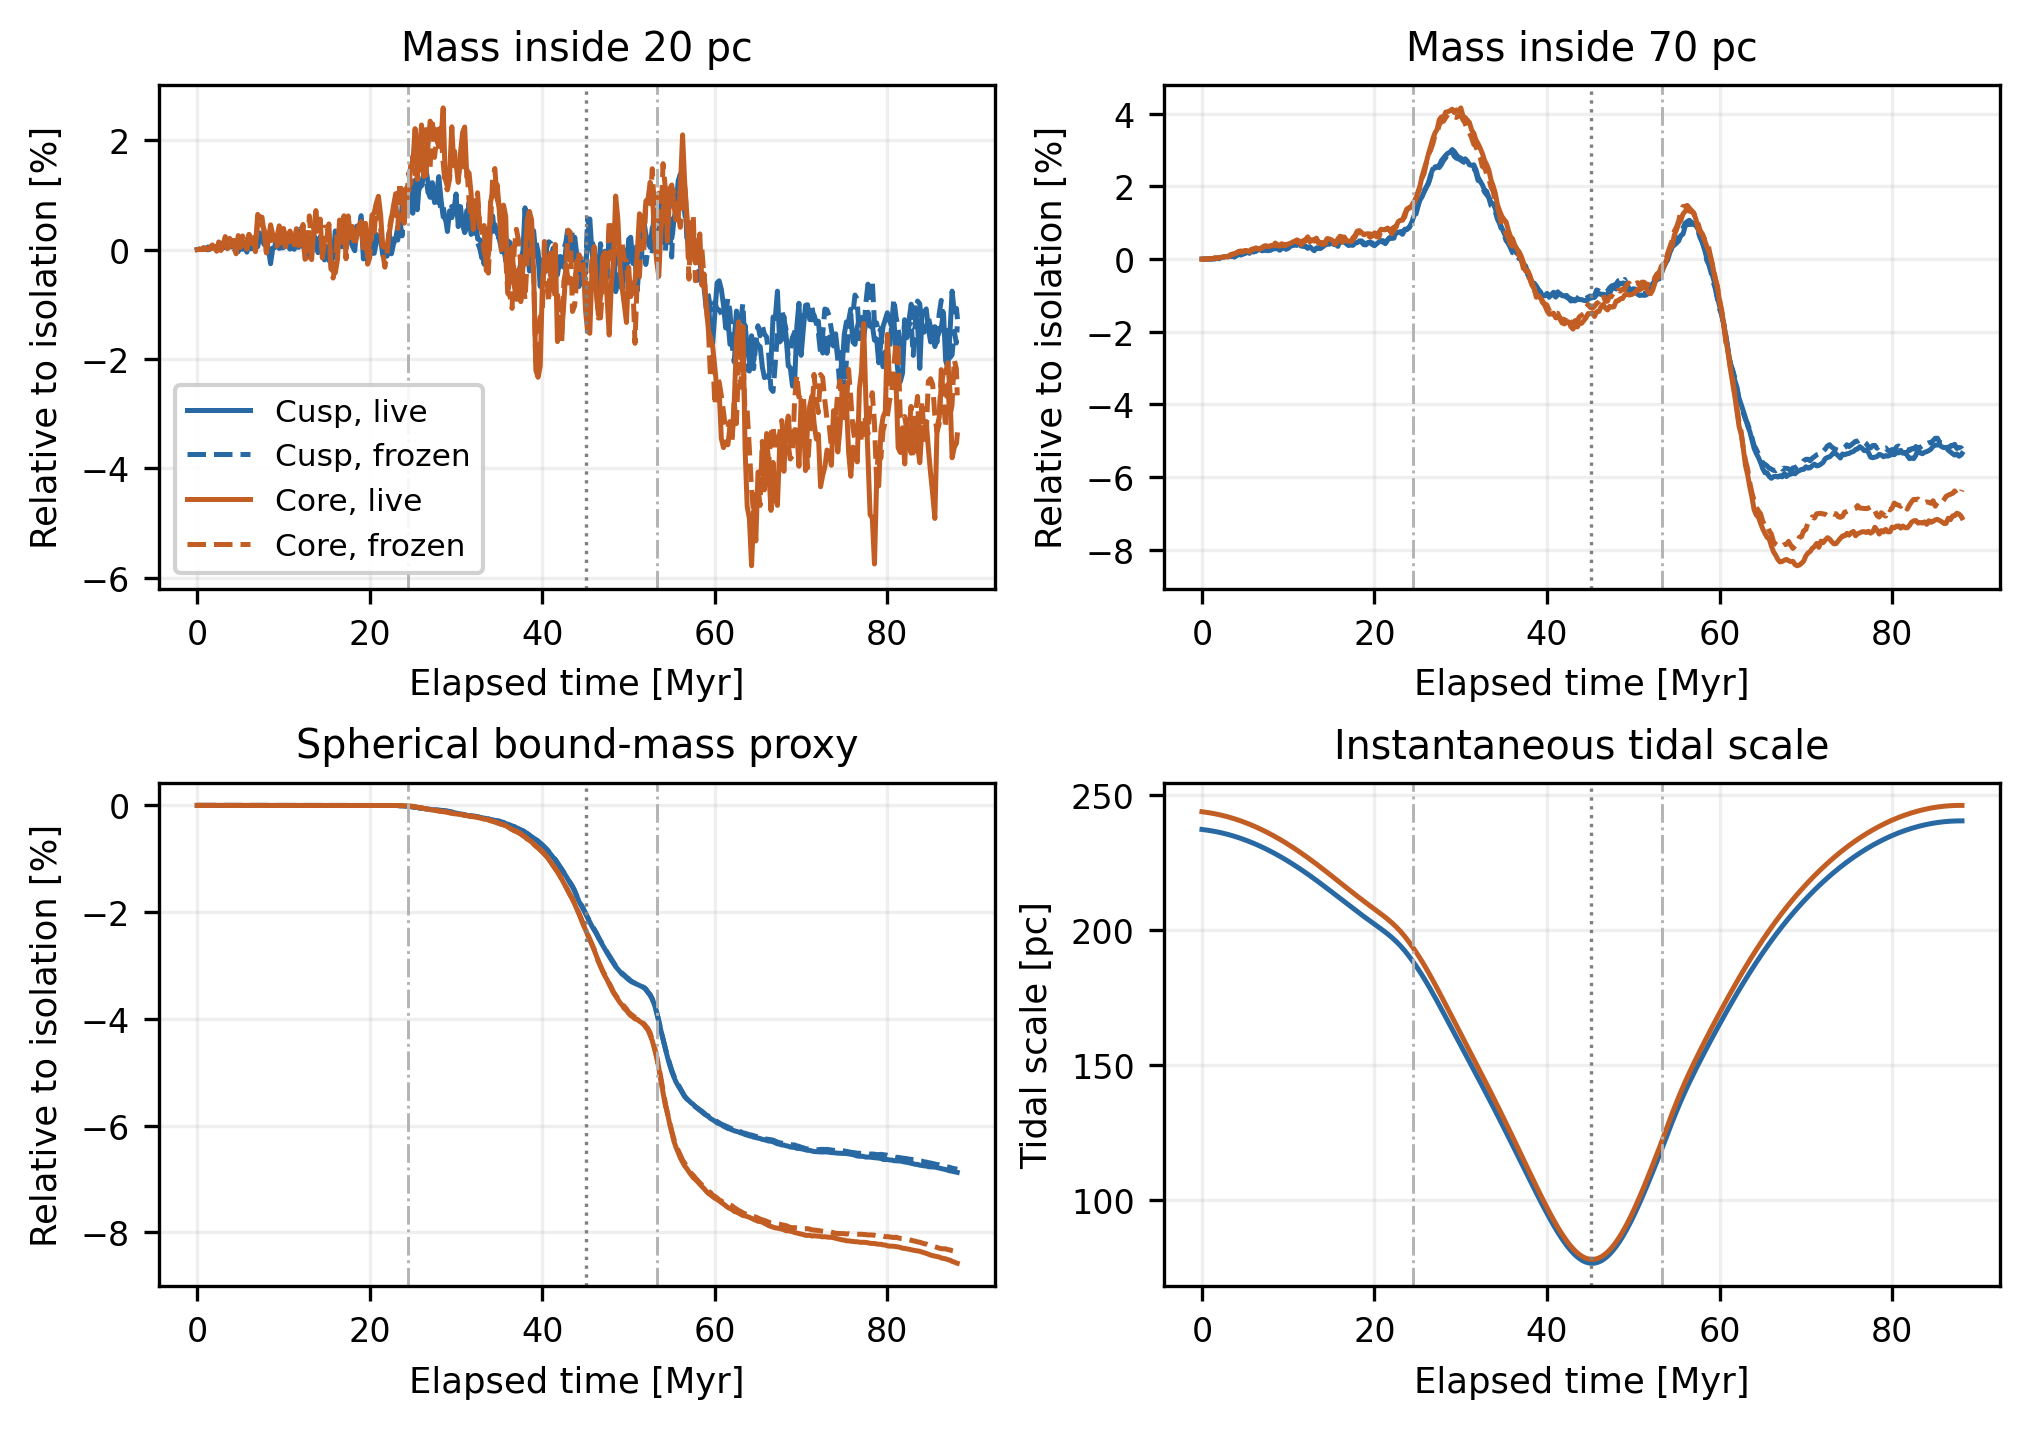
\includegraphics[width=\linewidth]{dynamical_batch_remnant_passage.png}
\caption{One Galactic passage for the compact cusp (blue) and core (orange).
Solid curves show live gravity; dashed curves show frozen potentials. The
three mass panels are relative to the corresponding full-interval isolation
control. The fourth panel shows the live instantaneous tidal scale. The dotted
vertical line marks pericentre; dot-dashed lines mark disc crossings. The
largest depletion occurs after the second crossing, while most central DM
remains.}
\label{fig:passage}
\end{figure}

The endpoint result persists across the final $10\Myr$. The live median
$20$-pc deficits are $1.41\%$ and $3.31\%$, with temporal 16th--84th percentile
ranges of $1.15$--$1.96\%$ and $2.43$--$4.02\%$.

Frozen medians are $1.43\%$
and $3.03\%$. Thus the net live/frozen difference is small compared with the
common tidal response at this stage. This is consistent with the compact
models being dominated centrally by the imposed nucleus. It does not show
that frozen gravity remains adequate after repeated stripping or for the
much more massive progenitors.

The final-10-Myr shell-density deficits relative to isolation are $2.50\%$
and $4.66\%$ at $20\pc$, increasing to about $17\%$ at $70\pc$ in both
profiles. The outer velocity distribution becomes tangential: median
$\beta(70\pc)=-0.298$ for the cusp and $-0.285$ for the core, compared with
values near zero in isolation. The $20$-pc distribution remains close to
isotropic. The $70$-pc shells retain thousands of effective particles;
the $3$-pc core shell falls as low as 59. Its large temporal excursions do
not establish a resolved central density change.

\begin{figure}[htbp]
\centering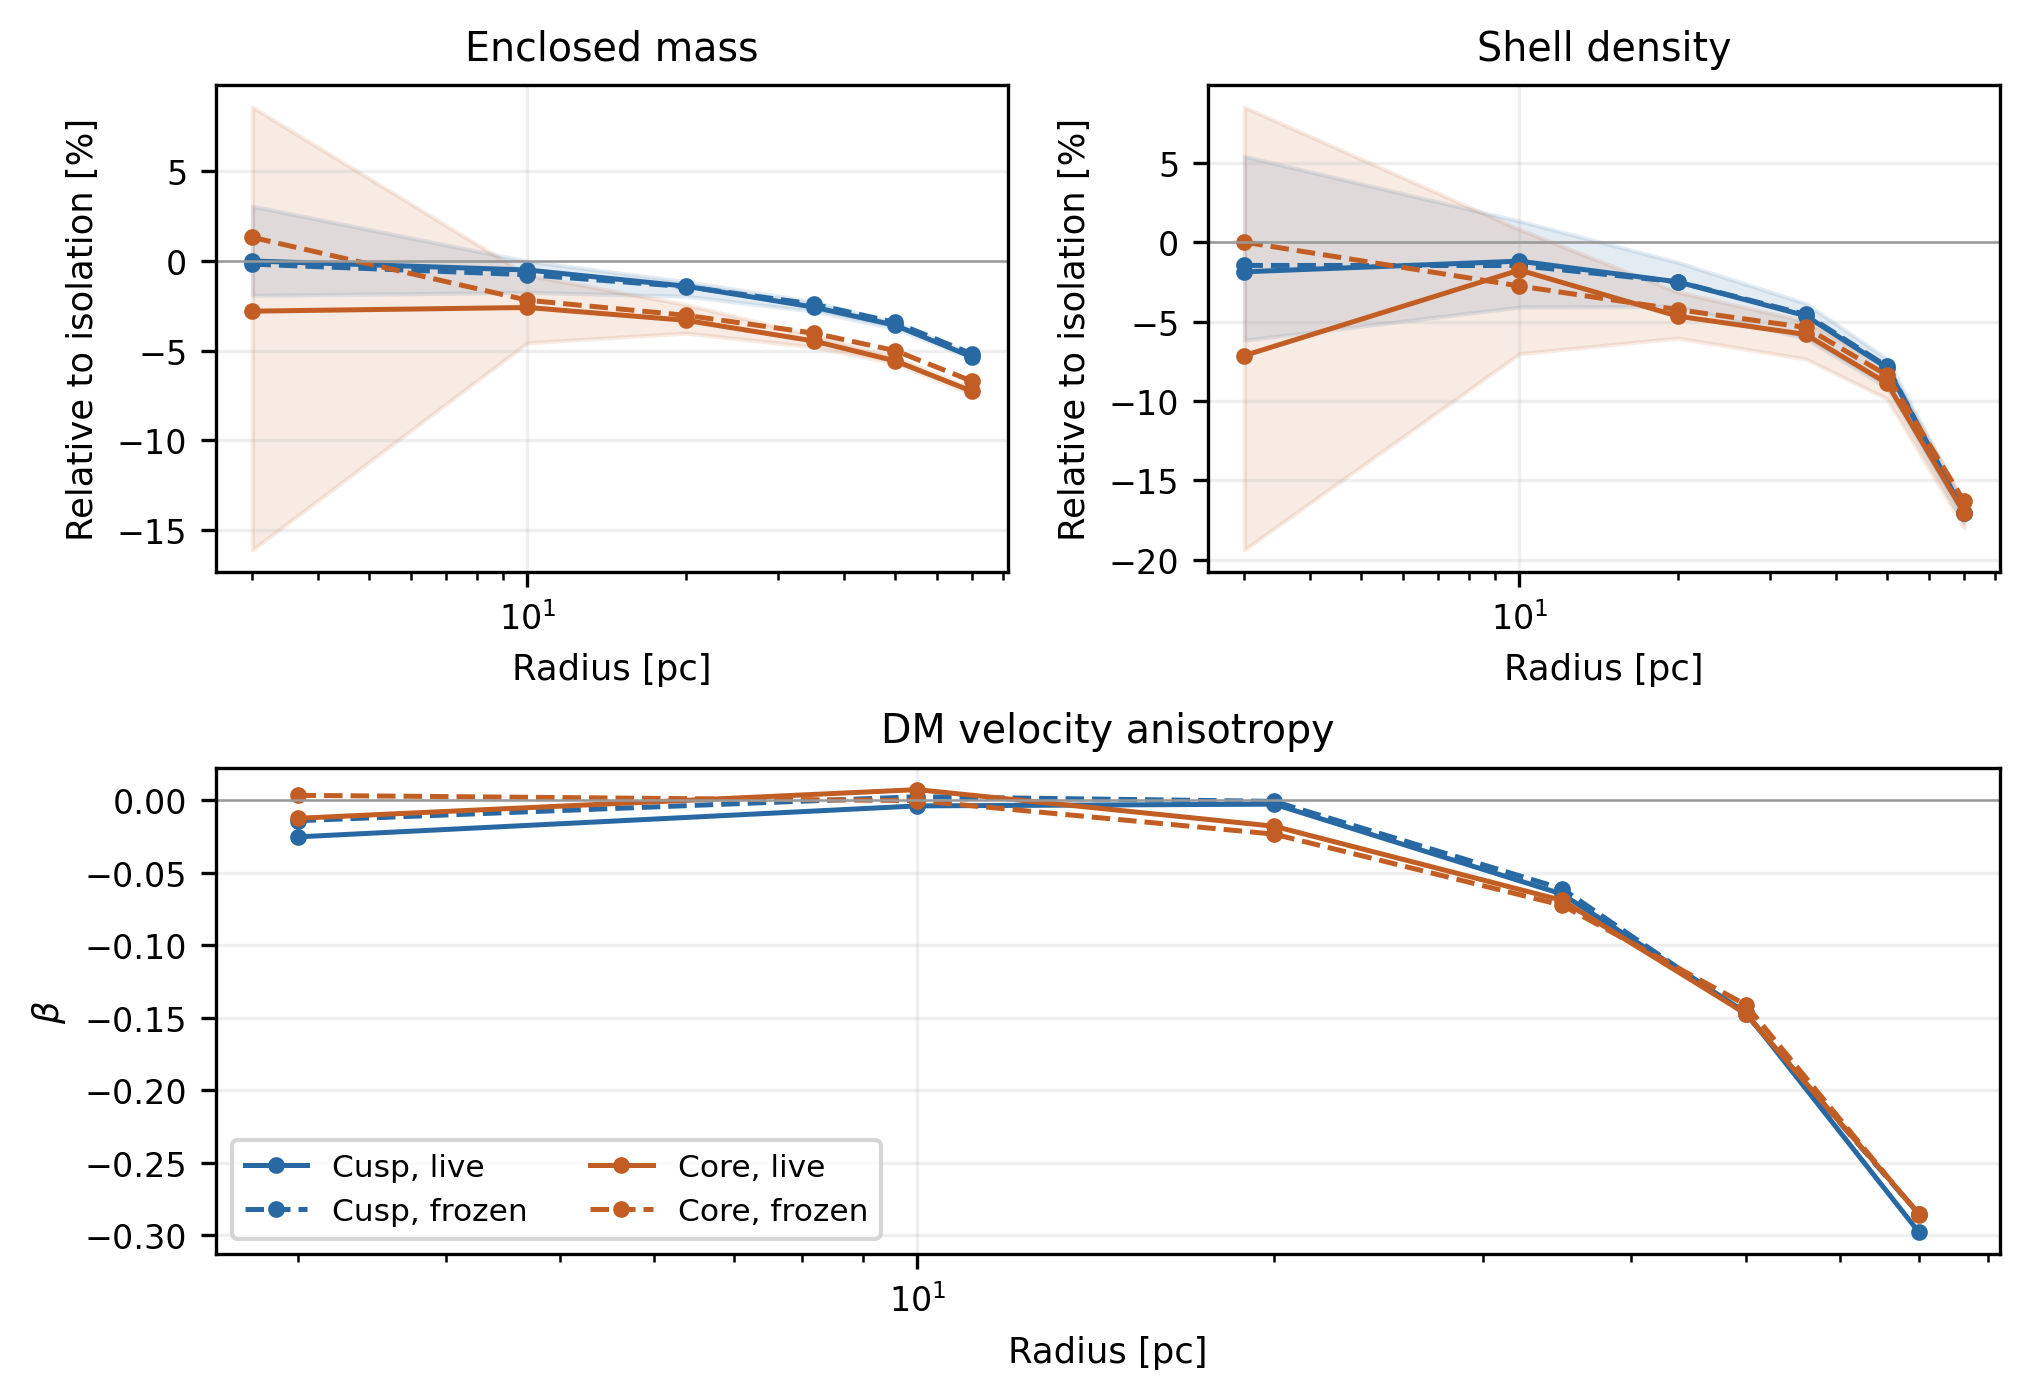
\includegraphics[width=\linewidth]{dynamical_batch_remnant_radial_response.png}
\caption{Radial response over the final $10\Myr$. The upper panels show median
enclosed-mass and shell-density changes relative to isolation; shaded regions
are the live temporal 16th--84th percentiles, not confidence intervals. The
lower panel shows median DM anisotropy in the tidal runs. Line styles and
colours follow Fig.~\ref{fig:passage}. The outer density and velocity
distribution change more strongly than the inner mass.}
\label{fig:radial}
\end{figure}

\FloatBarrier
\section{Disc crossings and the timing of heating}

The Cartesian track crosses the plane twice (Table~\ref{tab:events}). The
second crossing occurs $8.16\Myr$ after pericentre, at a smaller cylindrical
radius than the first. Its strongest compressive host-tensor eigenvalue has
magnitude about $0.0323\,\mathrm{Myr}^{-2}$, compared with
$0.0169\,\mathrm{Myr}^{-2}$ at the first crossing. The tidal scale in
equation~(\ref{eq:tidal}) instead reaches its minimum near pericentre:
$76.5\pc$ for the cusp and $77.9\pc$ for the core. These quantities describe
different parts of the tidal forcing; the minimum tidal scale alone does
not capture the compressive disc pulse.

\begin{table}[htbp]
\centering\small
\caption{Events on the saved orbit. Disc-crossing radii are cylindrical;
the pericentre radius is spherical. Times are measured from the initial
apocentre. Plane crossings were refined as roots of $z(t)=0$.}
\label{tab:events}
\begin{tabular}{lrrr}
\toprule
Event & Time [Myr] & Radius [kpc] & $v_z$ [km\,s$^{-1}$]\\
\midrule
First disc crossing & 24.42066 & 5.09361 & $-126.98$\\
Pericentre & 45.11369 & 1.99817 & ---\\
Second disc crossing & 53.27006 & 3.00873 & $+175.40$\\
\bottomrule
\end{tabular}
\end{table}

\begin{figure}[htbp]
\centering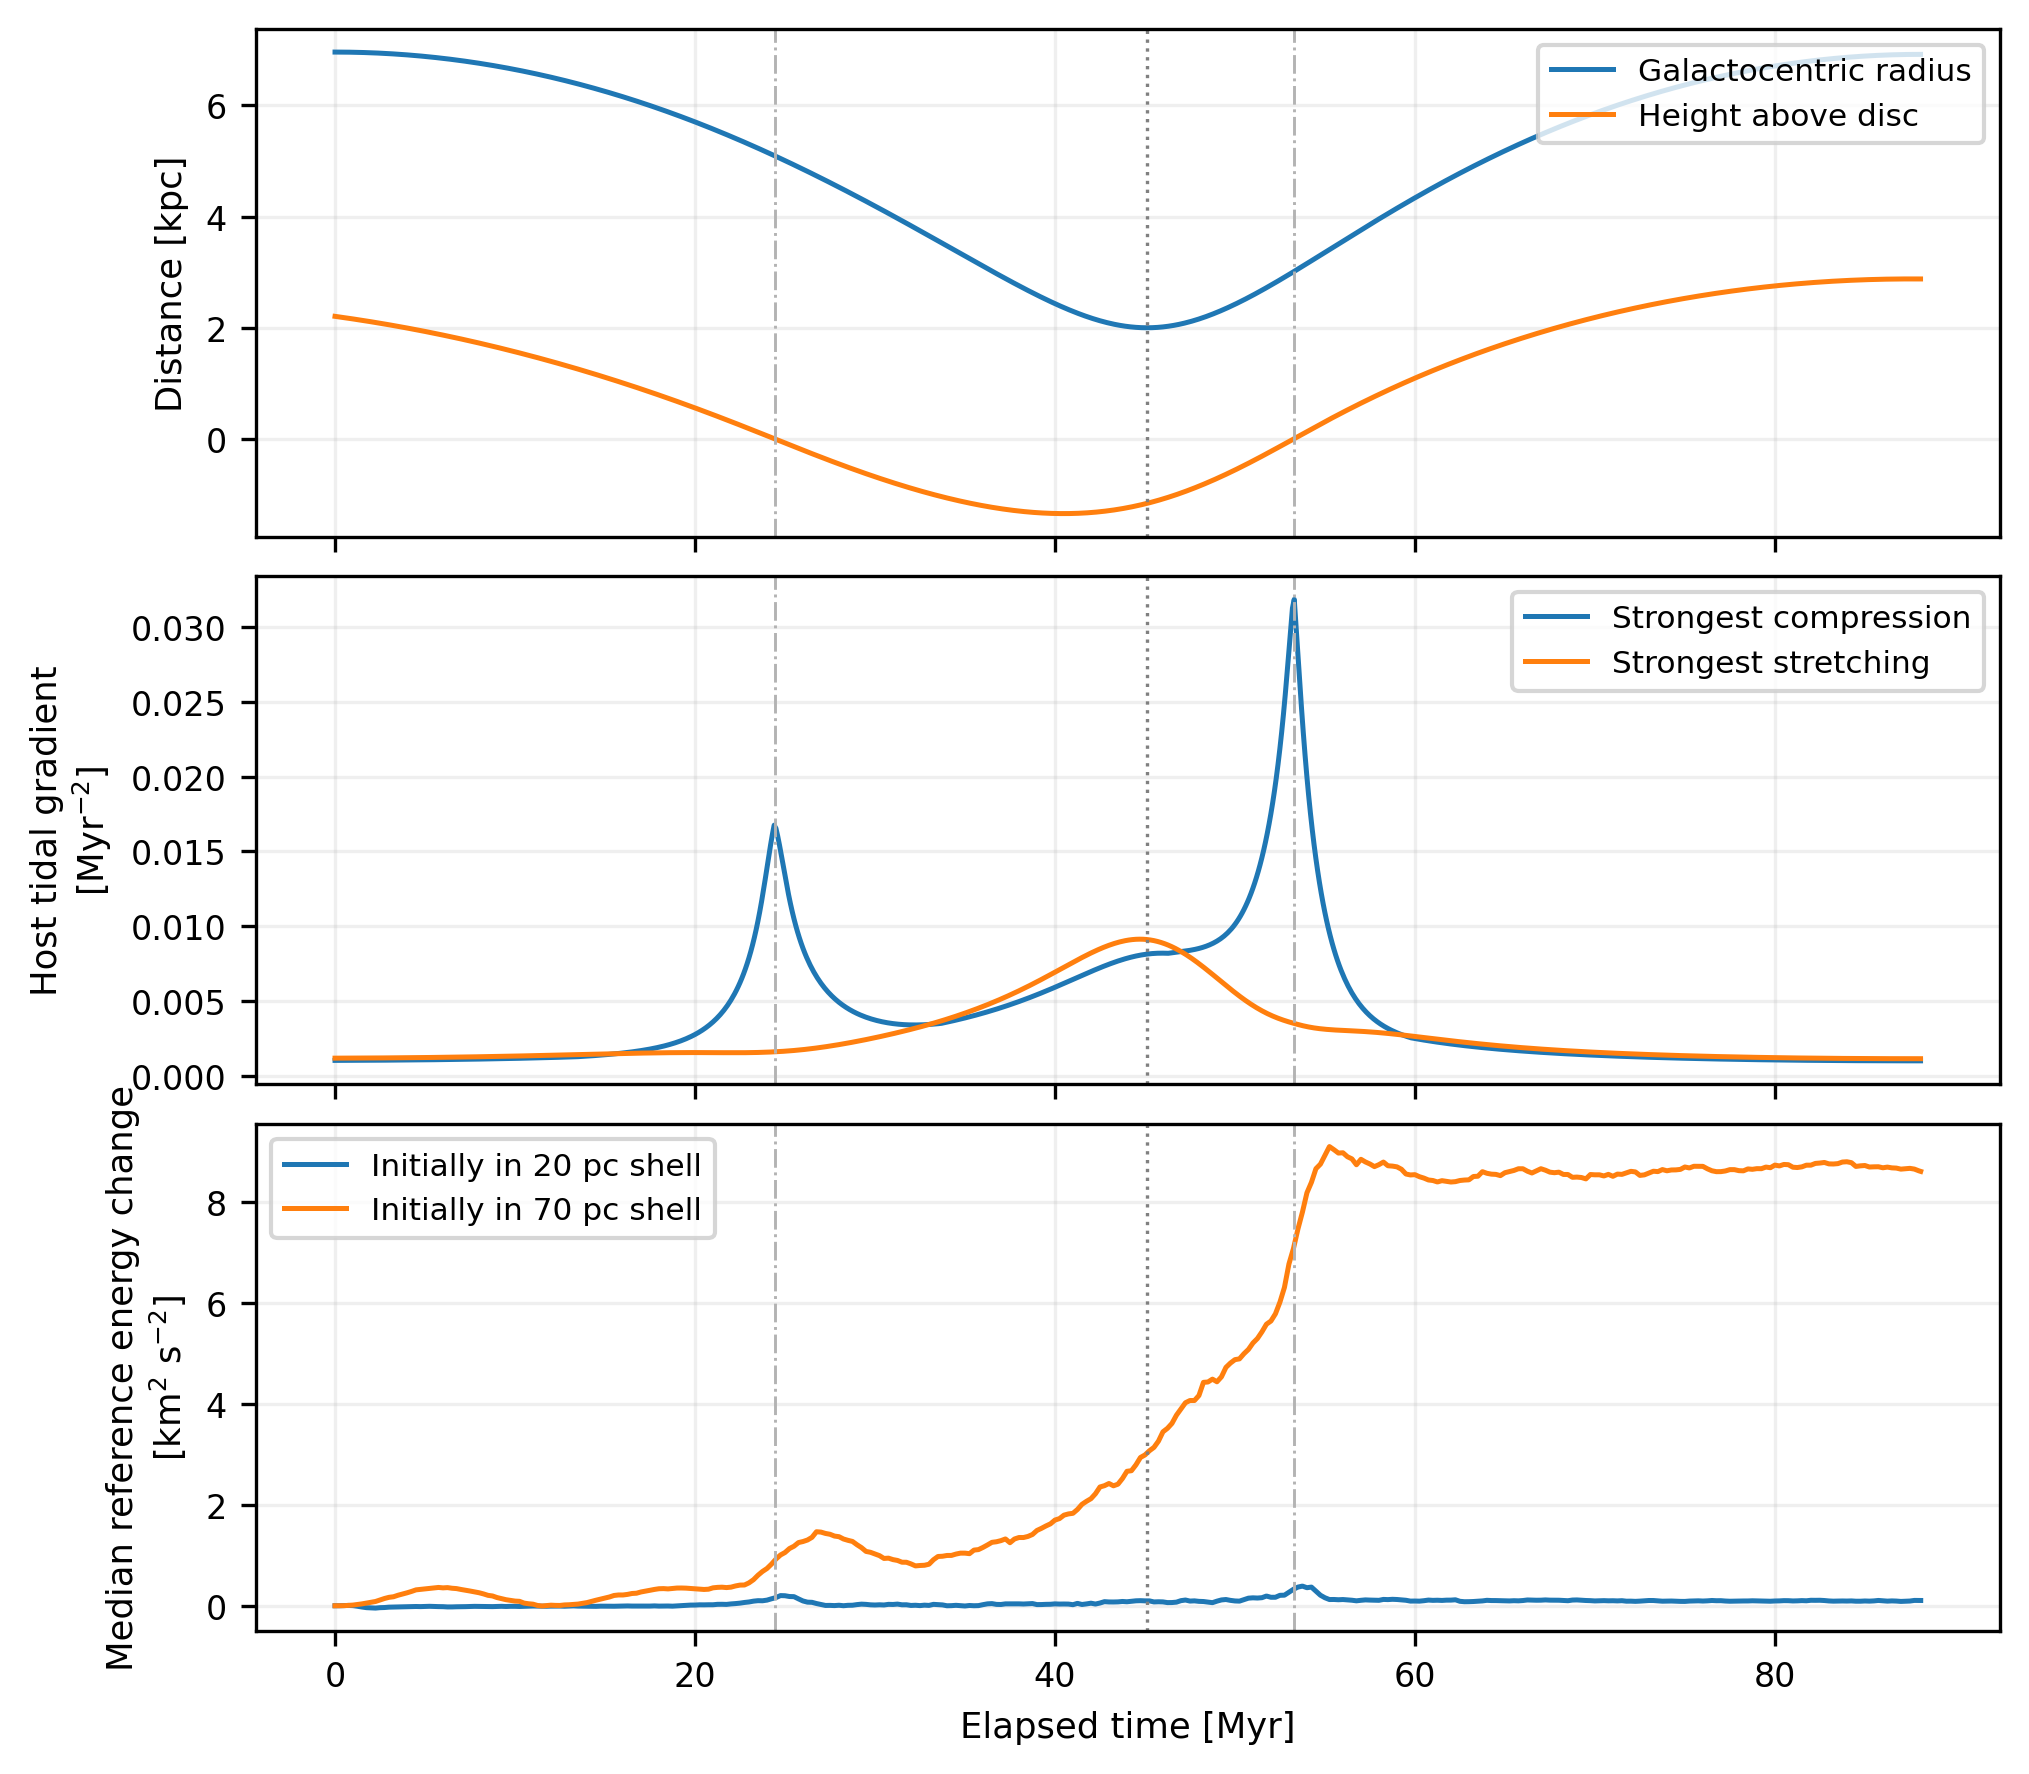
\includegraphics[width=\linewidth]{dynamical_batch_orbit_and_heating.png}
\caption{Orbit, host forcing and particle heating. Top: spherical
Galactocentric radius and height above the disc. Middle: the magnitudes of
the most compressive and most stretching eigenvalues of the inertial host
force gradient, without the centrifugal term. Bottom: median changes in the
initial-potential energy of frozen-cusp particles selected by their initial
$20$-pc or $70$-pc shells. The outer cohort heats much more strongly. Event
markers follow Fig.~\ref{fig:passage}.}
\label{fig:heating}
\end{figure}

The steepest decline in outer enclosed mass follows the second crossing
(Fig.~\ref{fig:passage}). In the frozen cusp, the final median
$\Delta E_{\rm ref}$ is $8.60\,\mathrm{km^2\,s^{-2}}$ for particles initially
in the $70$-pc shell and $0.104\,\mathrm{km^2\,s^{-2}}$ for the $20$-pc
cohort. The timing of the compressive pulse, outer heating and subsequent
depletion supports a contribution from disc shocking. This batch does not
contain a comparison that isolates the disc from the preceding pericentre
response, so it cannot assign their individual contributions.

\FloatBarrier
\section{Do the simulations agree with the analytical predictions?}
\label{sec:analytics}

There is qualitative agreement that the inner remnant changes less than its
outskirts, but neither simple analytical prescription gives a quantitative
prediction of this first passage. We compare density with density and energy
with energy below. An energy increment is not a predicted density decrement,
and a one-passage result cannot test a proposed many-Gyr equilibrium.

The earlier estimates in \path{docs/dm_capture_constraints.tex}, Section~11,
and \path{docs/SECTION11_TESTS.md} used representative pericentres. Here every
calculation uses the saved pilot orbit, with $r_{\rm p}=1.99817\kpc$ and
$v_{\rm p}=339.99\kms$, and the specified initial satellite model. The orbit
includes both disc crossings in Table~\ref{tab:events}. No new evolution was
launched for these comparisons.

\subsection{Density: instantaneous removal is too strong after one passage}

The original Kepler calculation removes all DF contributions with
$E>\Phi(r_t)$ from an isotropic, pure $r^{-\gamma}$ tracer around a point
mass. For $\gamma>1/2$ its retained density fraction is
\begin{equation}
 F_\gamma(x)=1-I_x(\gamma-1/2,3/2),\qquad x=r/r_t<1.
 \label{eq:kepler-cut}
\end{equation}
This is an energy cut, stricter than removing only orbits whose apocentre
exceeds $r_t$. Neither a Plummer-centred potential nor the tapered density
in equation~(\ref{eq:density}) satisfies its assumptions. In particular,
inserting $\gamma=0$ into this isotropic Kepler formula is invalid.

We therefore also calculate the energy cut using each actual isotropic
initial DF and its combined nucleus-plus-DM potential. With relative
potential $\Psi=-\Phi$, binding energy $\mathcal E=-E$, and
$\mathcal E_t=\Psi(r_t)$,
\begin{equation}
 \rho_{\rm cut}(r)=4\pi\int_0^{\sqrt{2[\Psi(r)-\mathcal E_t]}}
 v^2 f\!\left(\Psi(r)-\tfrac12v^2\right)\,\mathrm{d}v,
 \qquad r<r_t,
 \label{eq:actual-cut}
\end{equation}
and $\rho_{\rm cut}=0$ outside. The uncut density uses an upper limit
$\sqrt{2\Psi}$. We integrate both over the same finite shells as the
simulation diagnostics. The DF is not renormalised and the potential is not
updated after removal. Thus this is a specified instantaneous deletion
experiment, not a self-consistent equilibrium after stripping.

For a prediction independent of the measured mass loss, we evaluate the
tidal scale in equation~(\ref{eq:tidal}) with the \emph{initial} satellite
potential. Its minimum is $76.52\pc$ for the cusp and $78.01\pc$ for the
core. Figure~\ref{fig:analytic-density} compares this calculation with the
last-$10$-Myr median shell-density ratios. Table~\ref{tab:analytic-density}
lists representative radii.

\begin{table}[htbp]
\centering\small
\caption{Retained shell-density fractions. Simulation entries are relative
to matched isolation. The analytical energy cut uses the actual initial DF
and potential. These entries are density ratios, not enclosed-mass ratios.}
\label{tab:analytic-density}
\begin{tabular}{lrrrr}
\toprule
Profile & Radius [pc] & Live & Frozen & Energy cut\\
\midrule
Cusp & 20 & 0.9750 & 0.9750 & 0.8982\\
Core & 20 & 0.9534 & 0.9575 & 0.8529\\
Cusp & 50 & 0.9208 & 0.9217 & 0.5114\\
Core & 50 & 0.9110 & 0.9161 & 0.4926\\
Cusp & 70 & 0.8294 & 0.8291 & 0.1049\\
Core & 70 & 0.8295 & 0.8368 & 0.1190\\
\bottomrule
\end{tabular}
\end{table}

\begin{figure}[htbp]
\centering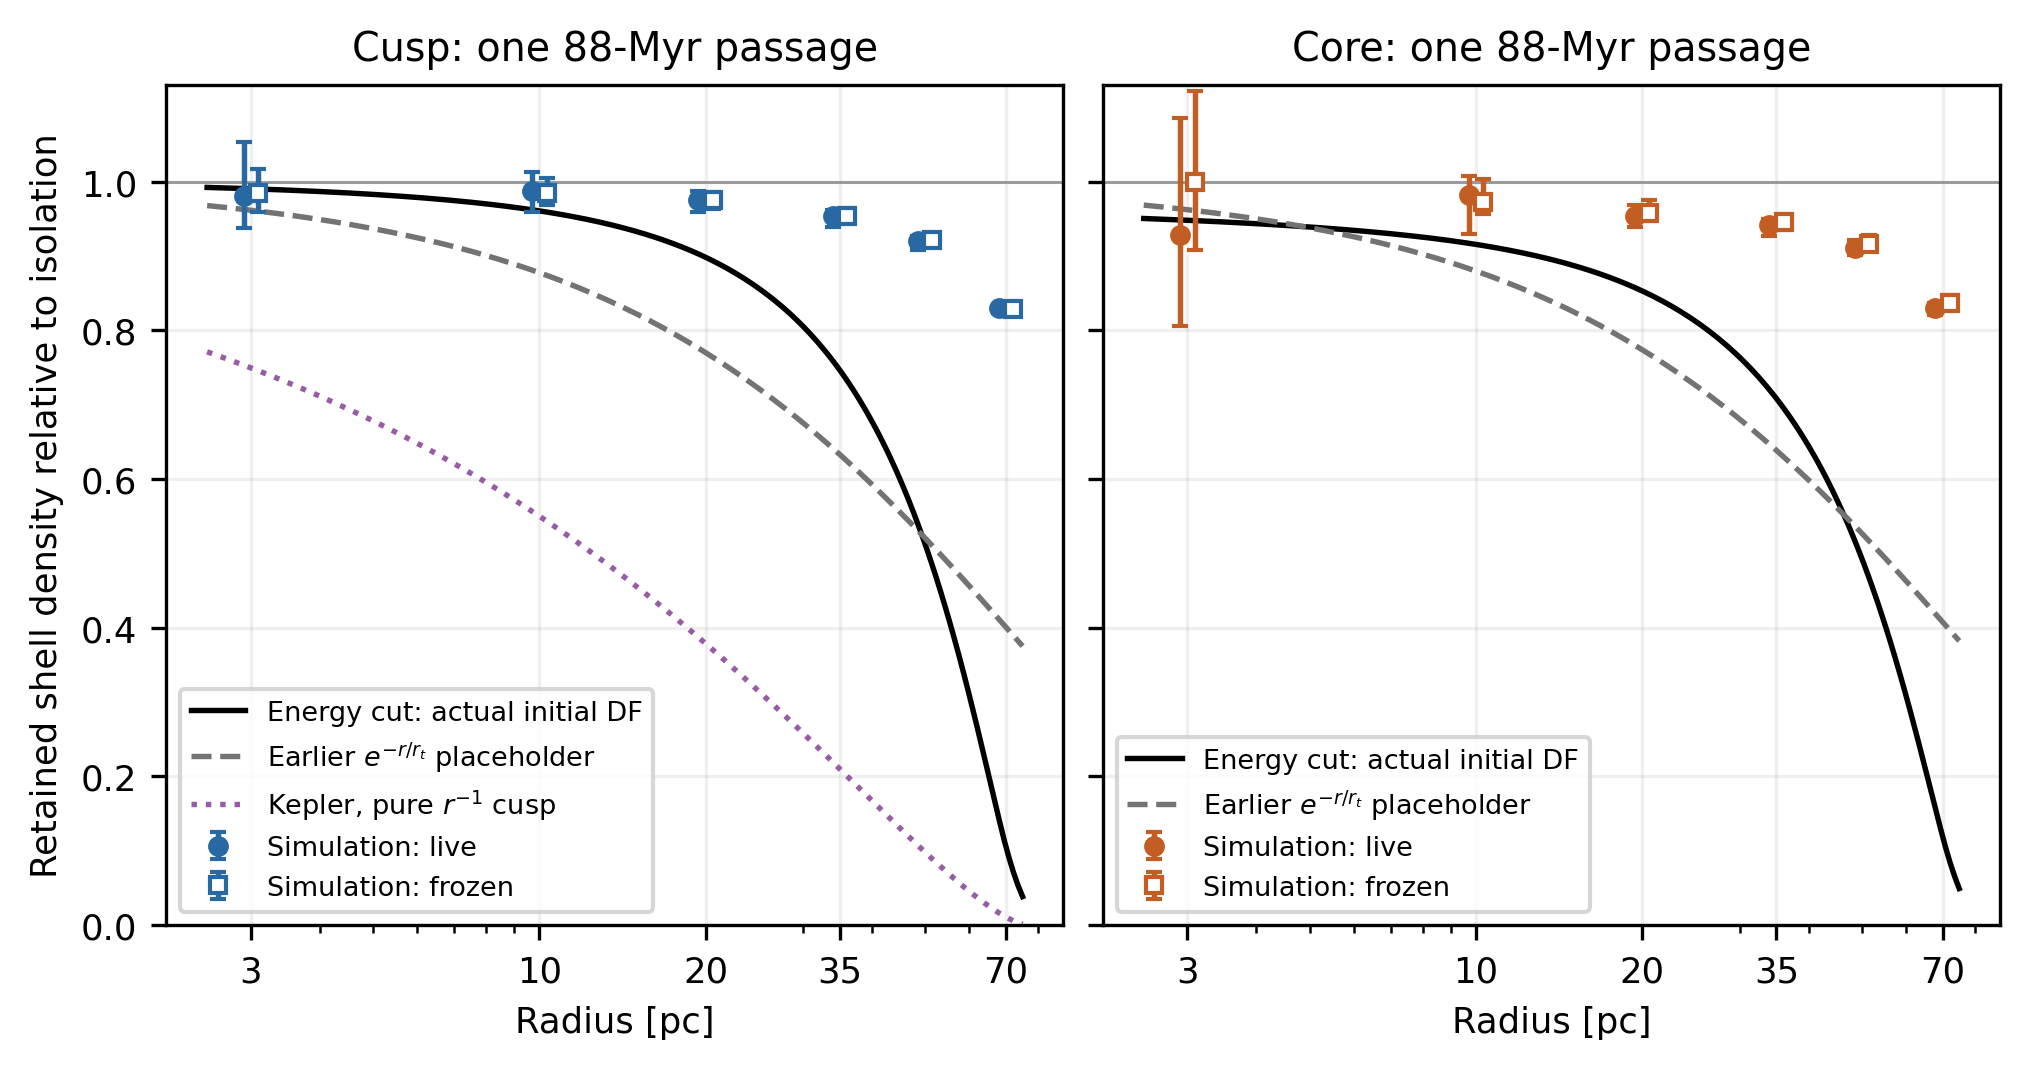
\includegraphics[width=\linewidth]{dynamical_analytics_density.png}
\caption{Density predictions and the measured first-passage response.
Filled circles and open squares show live and frozen results; bars give
temporal 16th--84th percentiles over the final $10\Myr$, not independent
statistical uncertainties. Points are offset slightly in radius for clarity.
The black curve deletes weakly bound phase space from the actual initial DF.
The dashed curve is the earlier exponential placeholder; the dotted curve
is the idealised Kepler $r^{-1}$ cusp, shown only for the cusp. The latter
two are pointwise reference prescriptions. None describes the measured
first-passage density profile quantitatively. The core at $3\pc$ is poorly
sampled, with as few as 59 effective shell particles during the passage.}
\label{fig:analytic-density}
\end{figure}

At $20\pc$, instantaneous removal predicts losses of $10.18\%$ and
$14.71\%$, compared with measured live losses of $2.50\%$ and $4.66\%$.
At $70\pc$, the predicted losses approach $90\%$, while the measured
losses are about $17\%$. Using the actual DF improves the comparison with
the idealised Kepler cusp, but does not make instantaneous removal a model
of the observed response. The Galactic tide varies, the remnant spends a
finite time near its minimum tidal scale, and an energy threshold discards
some angular-momentum-supported orbits confined within that scale. These
differences can account for stronger analytical depletion; their individual
contributions have not been isolated. Material outside the instantaneous
scale also need not escape immediately. The energy-cut curve is therefore
a useful reference for later evolution, not a demonstrated asymptotic state
or a rigorous bound on the density after many passages.

\subsection{Heating: the scalar pericentre estimate is too small}

The existing order-of-magnitude estimate uses
\begin{equation}
 \Delta v=T_{\rm p}r\tau,\qquad
 \tau=r_{\rm p}/v_{\rm p},\qquad
 \omega^2=GM_{\rm n}/r^3,\qquad
 A=(1+\omega^2\tau^2)^{-\gamma_{\rm ad}}.
 \label{eq:scalar-shock}
\end{equation}
For the flattened host we define its scalar radial-force analogue
$T_{\rm p}=-\boldsymbol a_{\rm host}\cdot\hat{\boldsymbol R}/r_{\rm p}$.
This corresponds to a force-equivalent spherical mass of
$1.904\times10^{10}\Msun$, rather than an exact enclosed mass of the
flattened model. The pilot gives $\tau=5.75\Myr$.
We adopt $\Delta E_{\rm pred}=\tfrac12(\Delta v)^2 A$ when plotting specific
energies. This makes the old dimensionless estimate
$(\Delta v)^2 A/(GM_{\rm n}/r)$ correspond to the characteristic energy
$GM_{\rm n}/(2r)$; it does not equate that scale to every particle's true
binding energy. Geometrical factors of order unity remain approximate.

The power-law adiabatic correction follows the shock calculations of
Gnedin, Hernquist \& Ostriker and Gnedin \& Ostriker
\cite{GHO1999,GO1999}. We show $\gamma_{\rm ad}=1.5$--$2.5$ as a sensitivity
range, not a fitted confidence interval. A scalar pericentre duration and
frequency do not describe the full host-tensor history, the two disc pulses,
or eccentric internal particle orbits.

To measure the response, we retain every particle selected by its initial
shell, including subsequent escapers, and compute in the frozen runs
\begin{equation}
 \Delta E_i=E_{i,\rm tide}(t_f)-E_{i,\rm isolation}(t_f),\qquad
 E_i=\tfrac12|\boldsymbol v_i-\boldsymbol V_{\rm n}|^2
       +\Phi_{\rm initial}(|\boldsymbol x_i-\boldsymbol X_{\rm n}|).
 \label{eq:matched-heating}
\end{equation}
Frozen potentials provide the cleanest comparison with an imposed-potential
estimate. The host can still do work and strip particles. The subtraction
removes the matched isolation drift. At $20\pc$ its mean energy change
has magnitude below $2.2\times10^{-5}\,\mathrm{km^2\,s^{-2}}$ throughout
the last $10\Myr$, far below the measured signal. We evaluate the analytical
prediction at every selected particle's initial radius before averaging.

\begin{table}[htbp]
\centering\small
\caption{Frozen full-orbit energy increments and the scalar pericentre
prediction with $\gamma_{\rm ad}=1.5$. Energies are in
$\mathrm{km^2\,s^{-2}}$. Means and medians refer to the same initial-shell
cohort. The last column uses its actual mean initial binding energy.}
\label{tab:analytic-energy}
\begin{tabular}{lrrrrr}
\toprule
Profile & Radius [pc] & Prediction & Mean & Median &
$\langle\Delta E\rangle/\langle|E_0|\rangle$\\
\midrule
Cusp & 20 & 0.00145 & 5.88 & 0.1045 & 0.0130\\
Core & 20 & 0.00147 & 6.46 & 0.1728 & 0.0150\\
Cusp & 50 & 0.402 & 17.29 & 2.134 & 0.0779\\
Core & 50 & 0.402 & 19.46 & 2.251 & 0.0834\\
Cusp & 70 & 2.257 & 37.52 & 8.602 & 0.2167\\
Core & 70 & 2.263 & 38.64 & 8.528 & 0.2102\\
\bottomrule
\end{tabular}
\end{table}

\begin{figure}[htbp]
\centering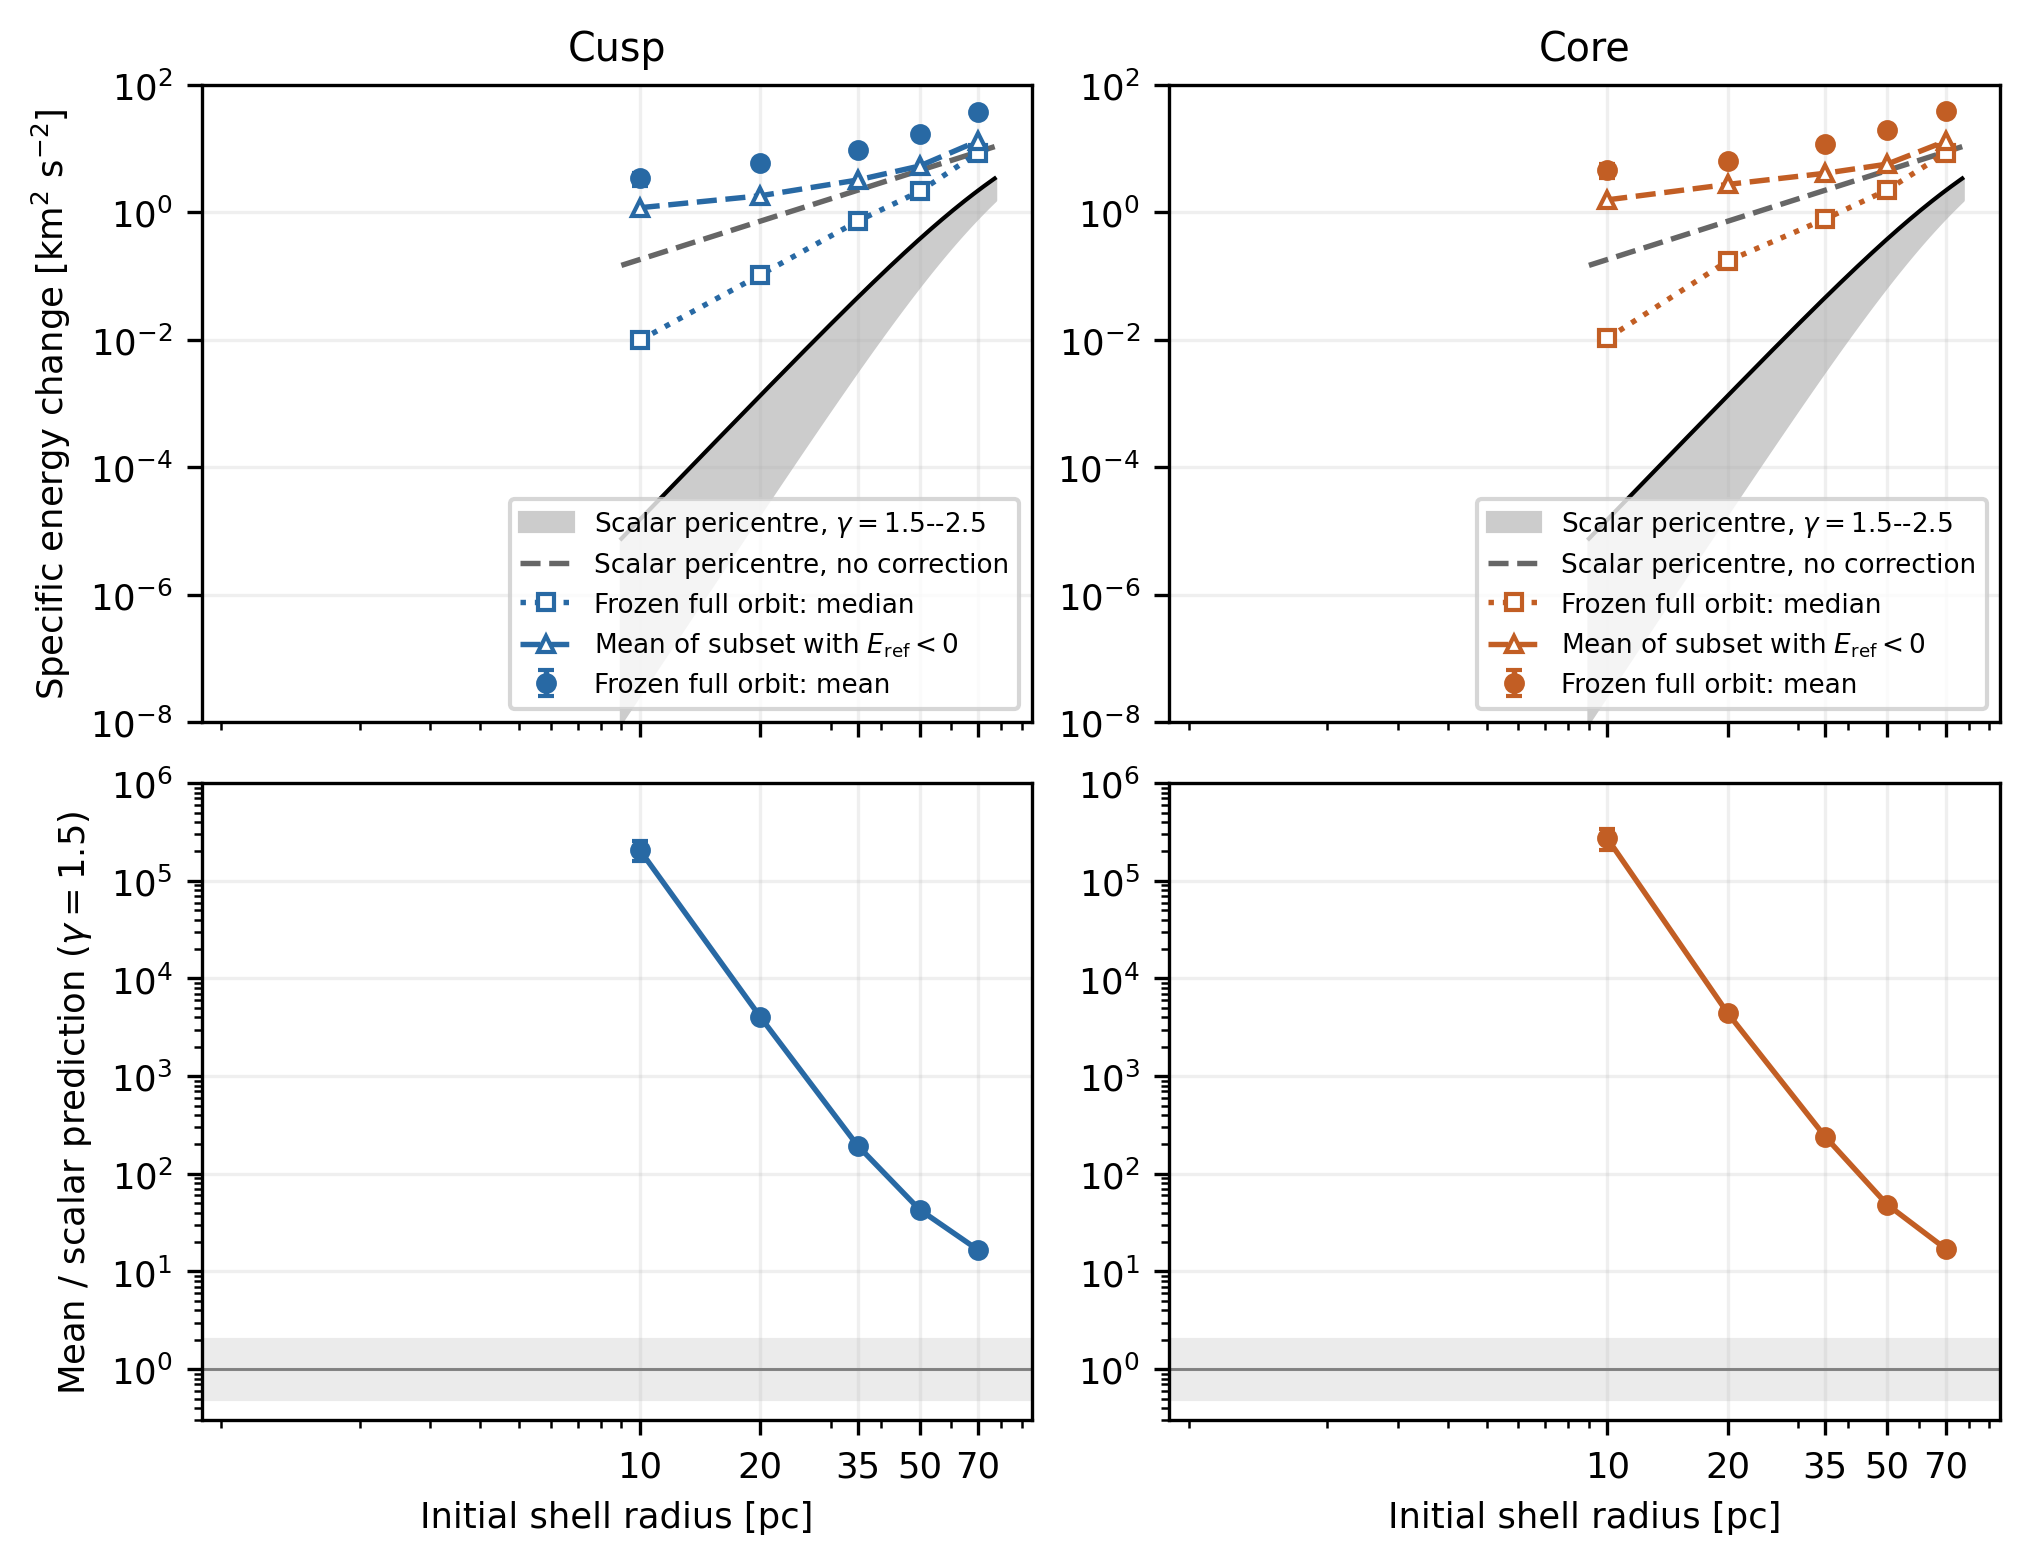
\includegraphics[width=\linewidth]{dynamical_analytics_heating.png}
\caption{Specific heating versus initial shell radius. Top: the scalar
pericentre estimate, with and without adiabatic suppression, compared with
the frozen full-orbit mean and median. Triangles restrict the mean to particles
with negative endpoint reference energy. Error bars on the mean are conditional
particle-sampling standard errors; they exclude modelling and convergence
uncertainty. Bottom: the mean divided by the shell-averaged prediction at
$\gamma_{\rm ad}=1.5$; the grey band denotes agreement within a factor two.
The $3$-pc shell is omitted because it lies inside the Plummer core, where
the assumed Kepler frequency is inappropriate. This figure tests the
adequacy of the scalar prescription for the full passage; it does not
isolate a pericentre shock from disc forcing or calibrate an adiabatic index.}
\label{fig:analytic-heating}
\end{figure}

The mean at $20\pc$ exceeds the corrected prediction by factors of about
$4050$ and $4400$. Even the medians exceed it by factors of $72$ and $118$.
At $70\pc$ the mean excess is about $17$. These discrepancies are much
larger than an omitted geometrical factor. Increasing $\gamma_{\rm ad}$
makes the prediction smaller. Thus the local, single-duration formula is
not calibrated by this batch, and fitting an exponent to the discrepancy
would mix different physical effects. In particular, the full-orbit mean
is not a measurement of heating by the pericentre alone.

The endpoint mean also includes continued host work on escaping particles.
Only about $1.1\%$ of either initial $20$-pc cohort has positive reference
energy at the endpoint, but those particles contribute $69\%$ of the cusp's
net energy increment and $58\%$ of the core's. Restricting the measurement
to negative reference energy gives mean increments of $1.82$ and
$2.75\,\mathrm{km^2\,s^{-2}}$, still far above the local prediction.
This is a selection diagnostic, not an exact bound/unbound classification
in the Galactic field. An endpoint cohort mean should not be interpreted
as heat retained by a closed, bound subsystem.

The large ratio to a very small analytical prediction does not imply
destruction of the inner remnant. The $20$-pc cohort's mean energy increment
is only $1.30\%$ or $1.50\%$ of its mean initial binding energy, while its
median increment is much smaller still. At $70\pc$ the corresponding
mean fractions are $21.7\%$ and $21.0\%$. These energy fractions belong to
fixed particle cohorts; the density measurements count whichever particles
occupy a shell at the later epoch.

\subsection{Why a particle at 20 pc is not a 20-pc orbit}

We compute each particle's apocentre in the initial spherical potential,
before applying the host. Among particles initially in the $20$-pc shell,
$28.7\%$ of cusp particles and $38.2\%$ of core particles have apocentres
beyond $40\pc$. Fractions of $7.1\%$ and $9.5\%$ reach beyond the minimum
tidal scale. Their larger excursions expose them to stronger differential
forces than a calculation that keeps them at $20\pc$.

Splitting the initial cohort at an apocentre of $40\pc$ makes this explicit.
Over the last $10\Myr$, the mean increments for confined orbits are
$0.083$ and $0.015\,\mathrm{km^2\,s^{-2}}$ for cusp and core. The means
for the more extended orbits are $18.38$ and
$15.74\,\mathrm{km^2\,s^{-2}}$. Weighted by their cohort fractions, these
extended orbits supply $99$--$100\%$ of the mean increment.
They also explain why the mean greatly exceeds the median. This comparison
averages increments per particle over saved outputs, so its values differ slightly
from the endpoint entries in Table~\ref{tab:analytic-energy}.

\begin{figure}[htbp]
\centering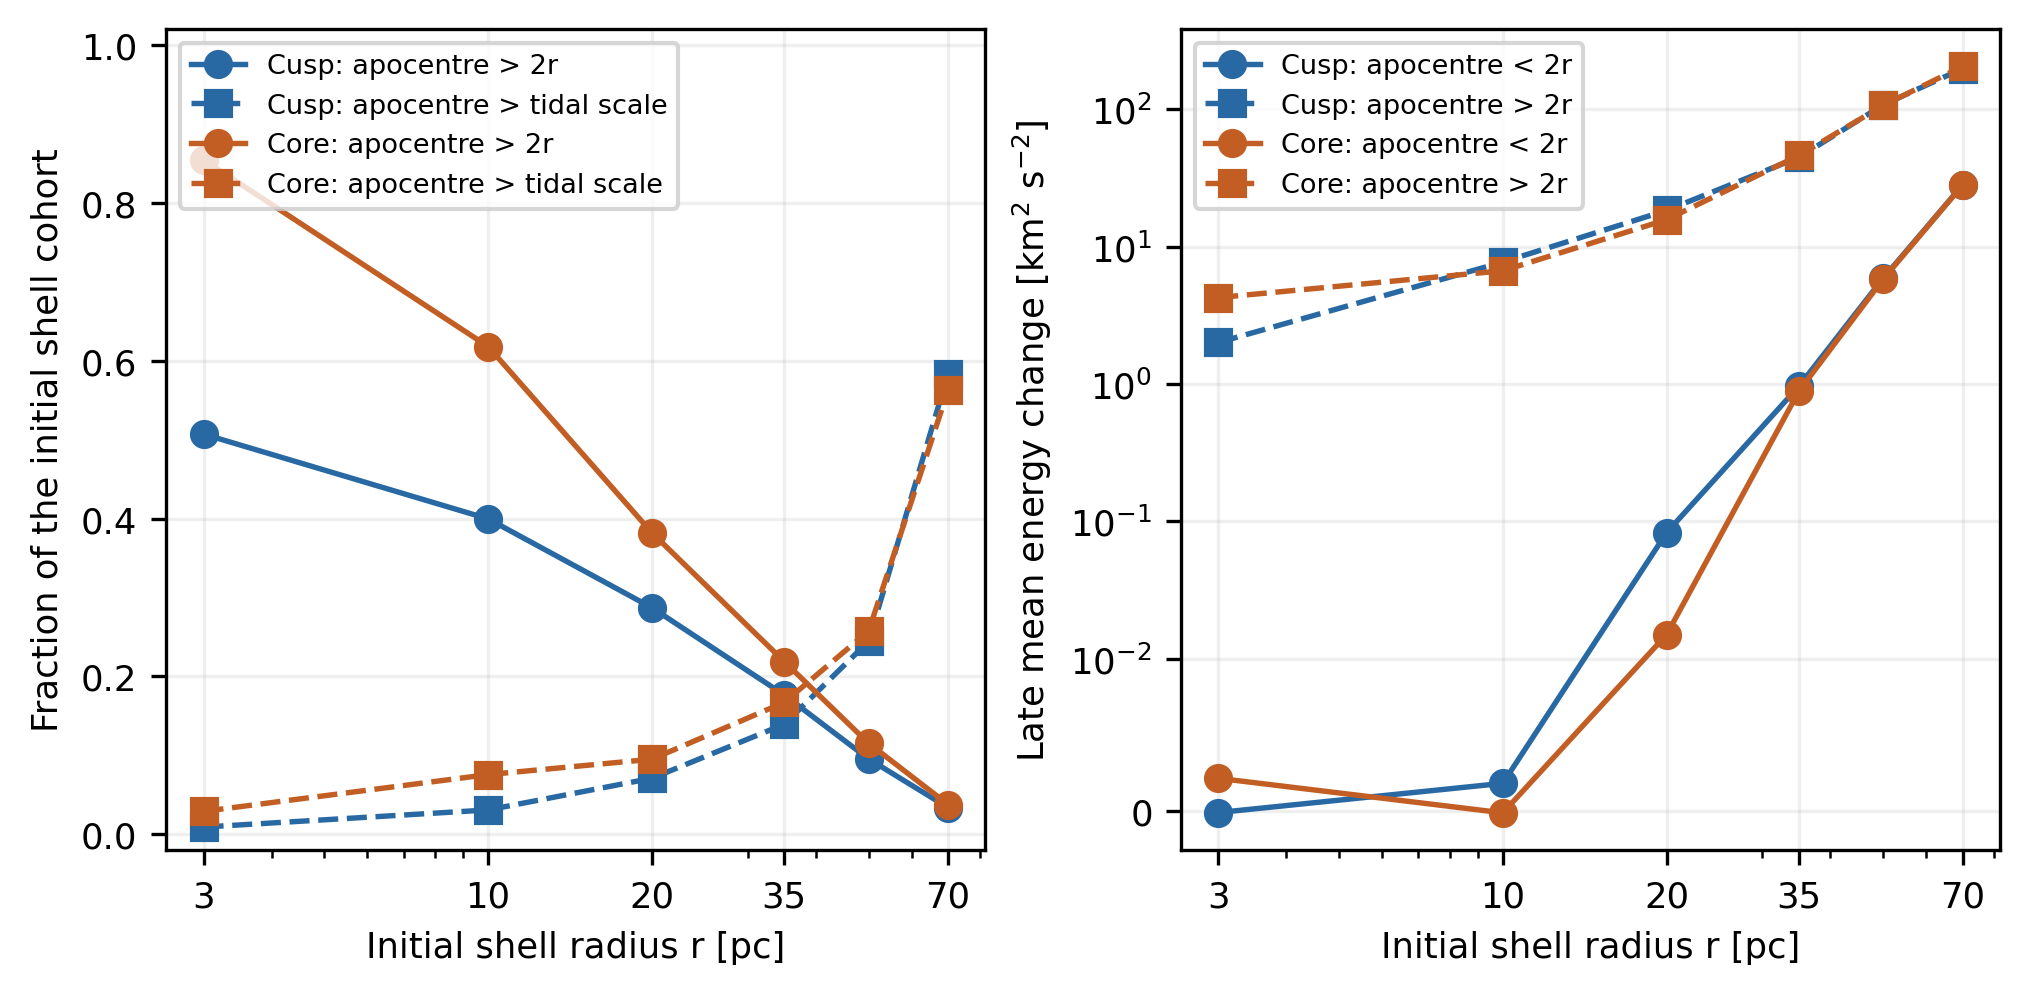
\includegraphics[width=\linewidth]{dynamical_analytics_orbital_cohorts.png}
\caption{The initial shell radius does not fix an orbit's radial extent.
Left: fractions of each initial cohort with apocentres beyond twice the
shell radius or beyond the minimum tidal scale. Right: mean frozen
tidal-minus-isolation energy increments, averaged over the final $10\Myr$,
split by initial apocentre. Extended orbits dominate the mean heating of
the inner cohorts. The right axis is linear very close to zero and
logarithmic away from zero. Lines connect the measured cohorts.}
\label{fig:analytic-cohorts}
\end{figure}

The observed hierarchy of inner and outer response therefore agrees with
the broad physical expectation. Quantitative agreement requires a prediction
that follows the actual internal orbits and time-dependent tidal tensor,
including the disc crossings and delayed escape. The present comparison
does not determine a unique disc contribution, an asymptotic retained
density, or a lifetime survival probability. Those remain questions for
the repeated-passage experiments and their numerical controls. The physical
stellar-heating timescale is also a separate prediction: these collisionless
runs do not simulate diffusion by real stars and cannot validate that rate.

\FloatBarrier
\section{Numerical sensitivity and the force-kernel repair}

The $20.00762\Myr$ isolation controls vary timestep, softening and particle
number separately. The first two comparisons retain the same initial phase
space and masses. Their endpoint $\Mtwenty$ differences are at most $0.116\%$
(Table~\ref{tab:controls}). The doubled-$N$ runs use different samples; their
own live/frozen differences are $+0.011\%$ for the cusp and $-0.155\%$ for
the core. Their offsets from the baseline should therefore not be interpreted
as pure numerical bias. All these isolation runs retain their initial bound
DM mass proxy.

\begin{table}[htbp]
\centering\small
\caption{Short-control endpoint $\Mtwenty$ differences from the original
live baseline, and maximum logged energy drift. Energy entries are
$100\max_t |[E(t)-E(0)]/E(0)|$. The half-softening cusp uses the repaired
force kernel.}
\label{tab:controls}
\begin{tabular}{lrrrr}
\toprule
 & \multicolumn{2}{c}{Mass difference [\%]} & \multicolumn{2}{c}{Energy drift [\%]}\\
\cmidrule(lr){2-3}\cmidrule(lr){4-5}
Control & Cusp & Core & Cusp & Core\\
\midrule
Baseline & --- & --- & 0.02930 & 0.01677\\
Half timestep & $+0.116$ & $-0.062$ & 0.00617 & 0.00266\\
Half softening & $+0.091$ & $+0.031$ & 0.01571 & 0.00696\\
Double particle number & $-0.642$ & $-0.046$ & 0.02942 & 0.01652\\
\bottomrule
\end{tabular}
\end{table}

\begin{figure}[htbp]
\centering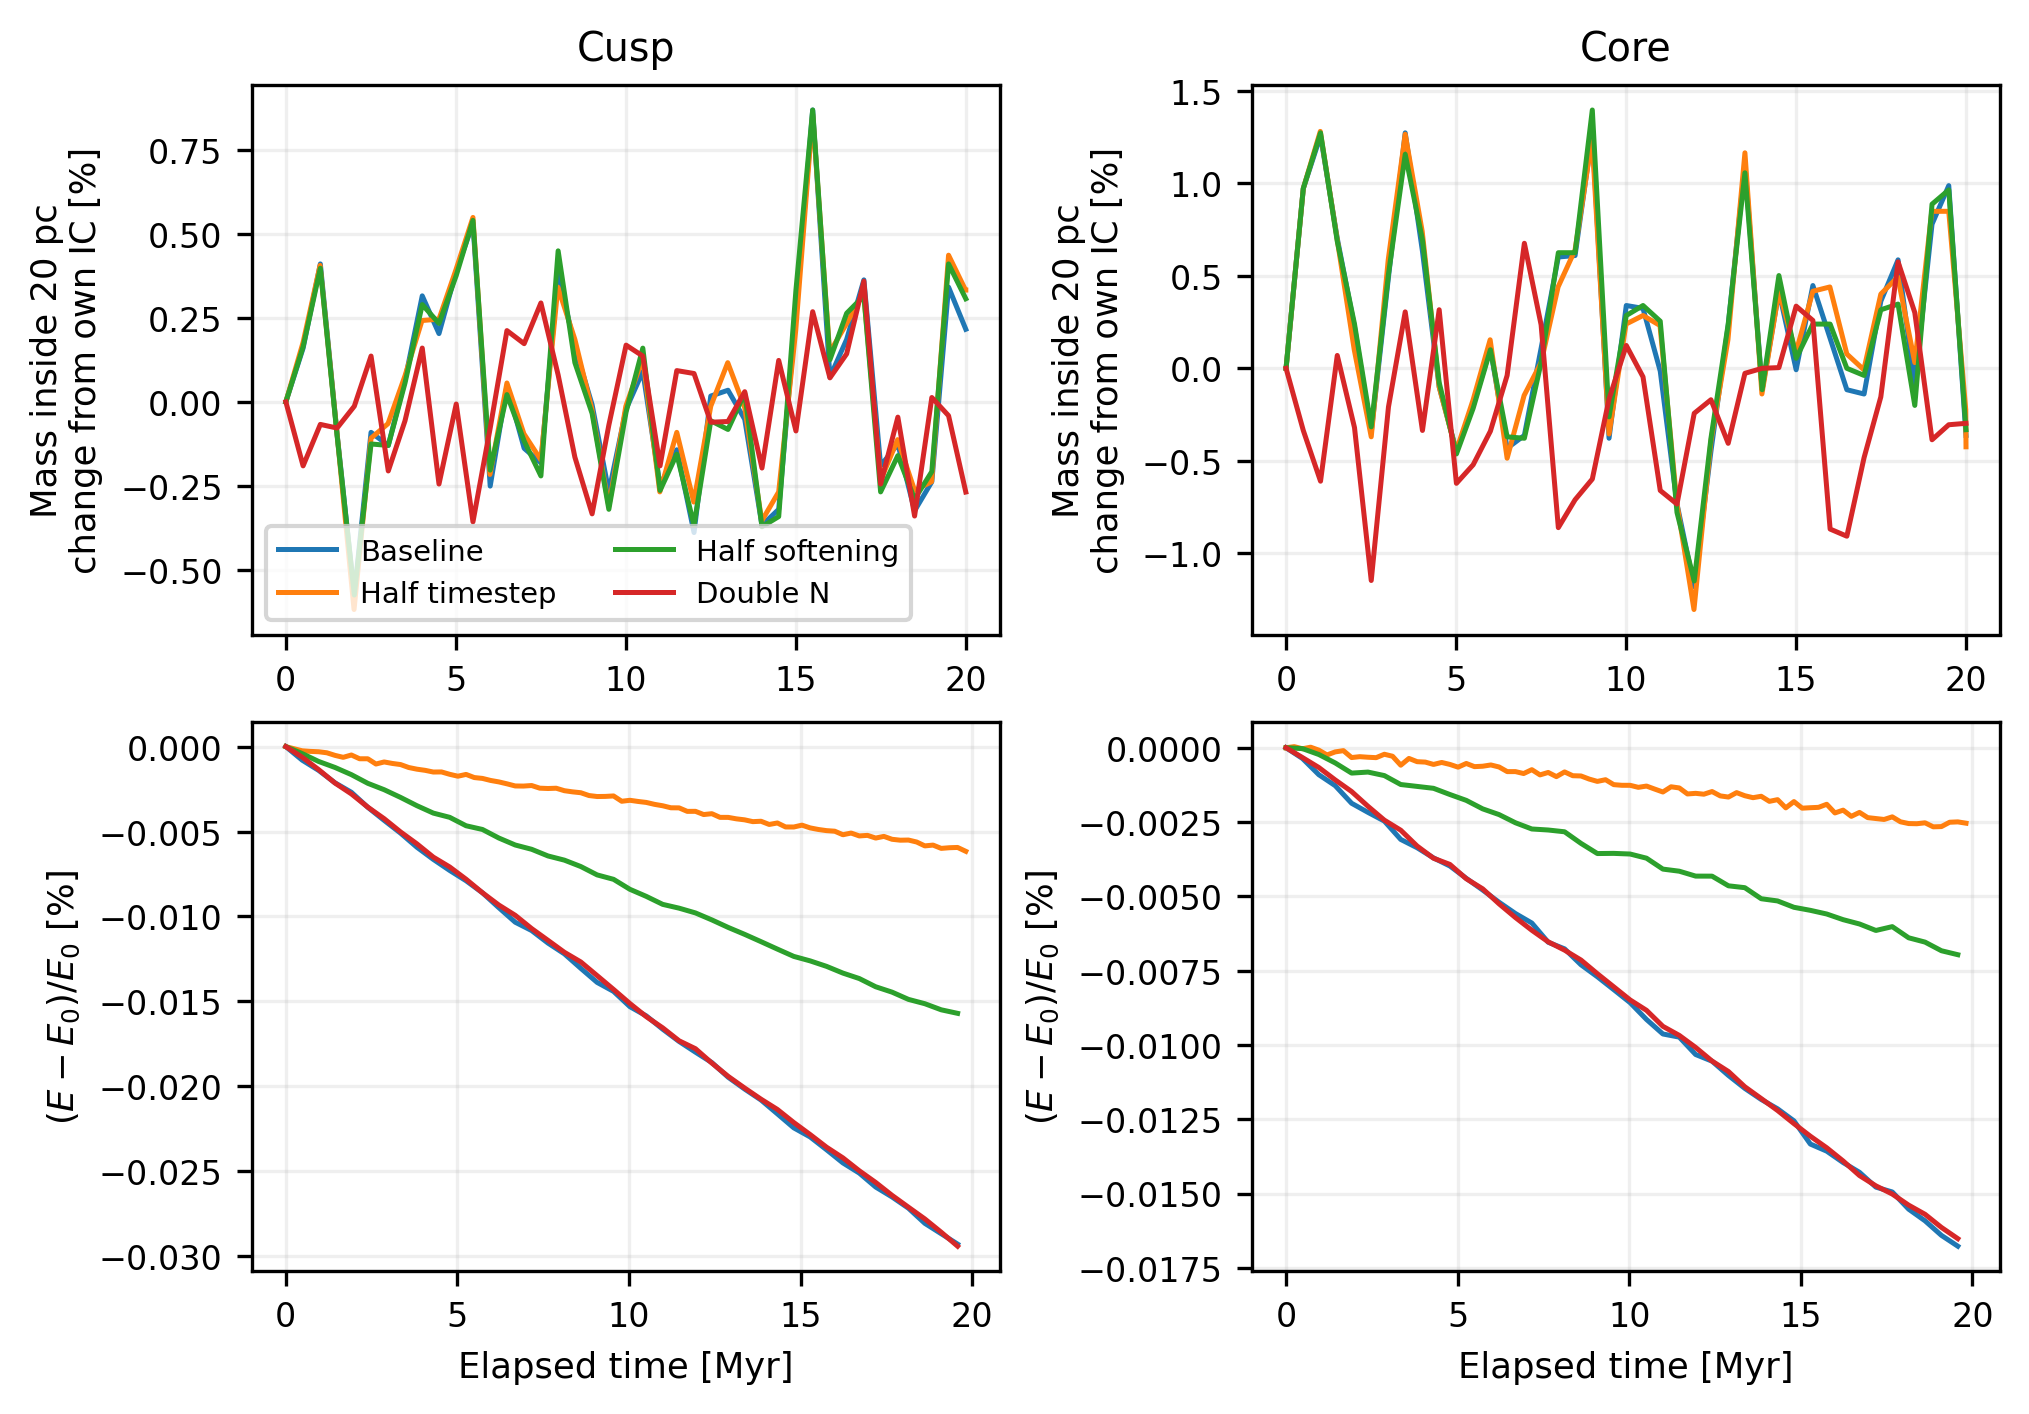
\includegraphics[width=\linewidth]{dynamical_batch_numerical_controls.png}
\caption{Remnant isolation sensitivity over $20\Myr$. Upper panels show
$\Mtwenty$ relative to each run's own initial sample, so they need not end
at the baseline differences in Table~\ref{tab:controls}. Lower panels show
logged energy changes; the same colour mapping applies in all panels.
Halving the timestep reduces the secular energy drift. The different
doubled-$N$ mass fluctuations include a change in particle realisation.}
\label{fig:controls}
\end{figure}

The longer baseline isolation runs reach maximum energy drifts of $0.135\%$
and $0.0728\%$ over $88\Myr$. Although their endpoint inner masses remain
stable, the secular trend favours the finer timestep for longer experiments.
No linear extrapolation of that drift to a many-Gyr integration is assumed.
The short controls support the pilot interpretation, but they have not tested
resolution sensitivity under the full $88$-Myr tidal forcing. There is also
only one sampling seed.

The initial cusp run with $0.1\pc$ softening failed because an intermediate
coefficient in the installed single-precision P1 Taylor kernel overflowed.
An unchanged repeat reproduced the failure.

With
$Q=r^2+\epsilon^2$ and $H=\epsilon^2/2$, the repaired implementation evaluates
the same coefficients as
\begin{equation}
 D_n=T_n\left[1+(2n+1)\frac{H}{Q}\right],\qquad
 T_n=M(2n-1)!!\,Q^{-n-1/2},
\end{equation}
without forming an unnecessary higher derivative that overflows before being
multiplied by $H$. Double-precision intermediates are used; native coefficients
that genuinely exceed range are rejected explicitly. The repair preserves
the force law, masses, softening and timesteps. A run-local library replaces
only the kernel object; the installed NEMO source and library are unchanged.

The original $10^5$-particle configuration then completed the full
$20.00762\Myr$, giving 41 analysed snapshots. A 64-particle close-cell
reproducer fails with the original library and passes with the repair, with
maximum force error $7.25\times10^{-5}$ relative to direct P1 summation.
The focused suite passed 95 tests, followed by five kernel/integrity tests
after the runtime checks were strengthened. The original failures and
instrumentation attempt remain preserved. Other completed batch runs used
the original kernel; the repaired kernel has not yet been used to repeat
the full tidal passage.

\FloatBarrier
\section{Extended progenitors in isolation}
\label{sec:progenitors}

Both progenitor pairs complete $100.00826\Myr$. Their DM and stellar bound-mass
proxies remain constant, with maximum logged live energy drifts of
$0.00244\%$ for the cusp and $0.00114\%$ for the core. At every saved epoch,
the fraction of mass inside the $100$-pc protection radius contributed by
particles heavier than ten times their component's minimum mass is zero.
This is the defined heavy-particle diagnostic; it does not exclude all
effects of the mass spectrum or finite-particle relaxation.

\subsection{Mass profiles on the scale of the extended body}

The original diagnostic apertures stop at $70\pc$. We therefore independently
read the final snapshots and extend the enclosed-mass measurements to
$100$, $200$, $500$, $1000$, $2000$, $5000$ and $10000\pc$.
At every one of these radii, the live and frozen endpoint masses agree within
$1\%$ for both components in both progenitors. At $1\kpc$, the DM differences
are $-0.38\%$ and $-0.53\%$, while stellar differences are $-0.35\%$ and
$-0.14\%$ for cusp and core, respectively.

\begin{figure}[htbp]
\centering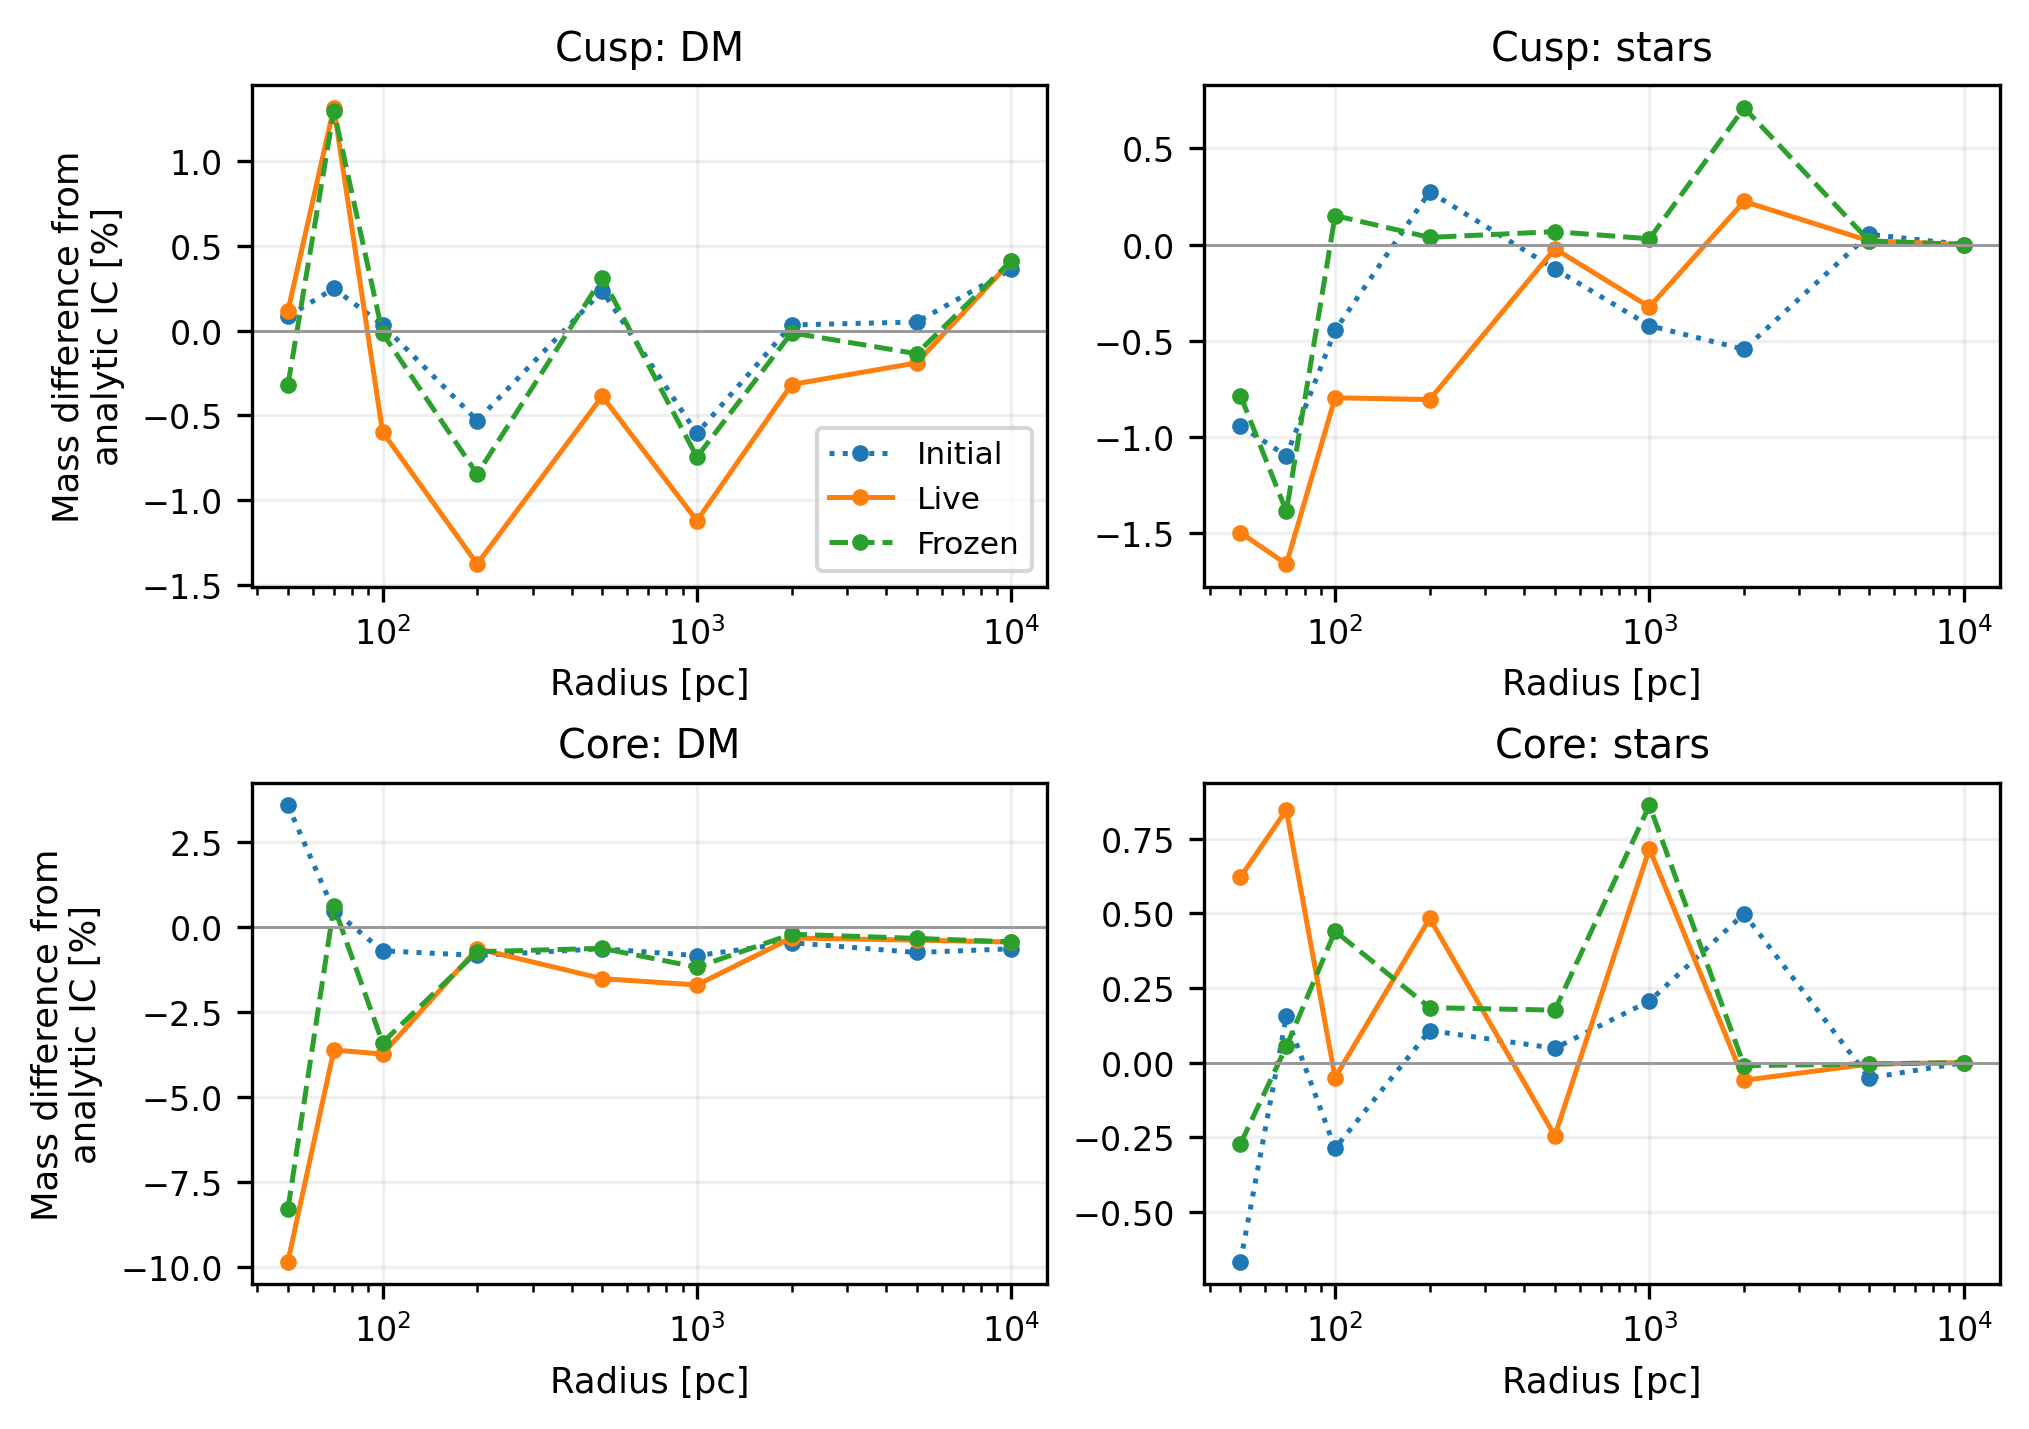
\includegraphics[width=\linewidth]{dynamical_batch_progenitor_global_profiles.png}
\caption{Progenitor enclosed masses relative to the analytic continuum IC
profile. Dotted lines show the initial particle sample; solid and dashed
lines show live and frozen endpoints at $100\Myr$. Both DM and stars remain
close on the scales of the extended body. The larger cored-DM fluctuations
at $50$--$100\pc$ must be read with the smaller effective counts. The plotted
offsets from the analytic model include initial sampling fluctuations.}
\label{fig:global}
\end{figure}

These endpoint comparisons support using the models for first experiments on
disruption of the extended body. They do not provide a complete time series
at those larger radii; the next runs should save diagnostics there at every
output time. The live/frozen agreement is a pilot stability check, not a
convergence demonstration across particle numbers or refinement schemes.

\subsection{Central particle counts and their consequences}

Central resolution differs strongly between profiles
(Table~\ref{tab:resolution}). The analytic cored DM mass inside $20\pc$ is
only $2772\Msun$, compared with $149950\Msun$ for the cusp. The initial core
sample contains 16 particles there, corresponding to $2142\Msun$; it was
already below the continuum target before evolution.

\begin{table}[htbp]
\centering\small
\caption{Initial central resolution of the progenitor models. DM particle
weights inside these apertures are equal, so the listed aperture effective
counts coincide with particle counts. Shells have width $\pm0.1$ in $\ln r$.}
\label{tab:resolution}
\begin{tabular}{lrr}
\toprule
Quantity & Cusp & Core\\
\midrule
Analytic $\Mtwenty$ [$\Msun$] & 149950 & 2772\\
Sampled $\Mtwenty$ [$\Msun$] & 152315 & 2142\\
DM $N_{\rm eff}$ inside $20\pc$ & 539 & 16\\
DM $N_{\rm eff}$ in the $20$-pc shell & 205 & 15\\
Stellar $N_{\rm eff}$ inside $20\pc$ & 669 & 692\\
\bottomrule
\end{tabular}
\end{table}

The core ends with 18 live and 23 frozen DM particles inside $20\pc$.
Expressed relative to its initial sample, these become apparent mass increases
of $12.5\%$ and $43.75\%$. Both series fluctuate strongly and both have a
median aperture count of 20. These percentages do not establish physical
central growth. Its shell density and anisotropy are also poorly sampled.
The cusp's several hundred central DM particles can reveal gross changes,
but small shell-density differences remain noisy.

\begin{figure}[htbp]
\centering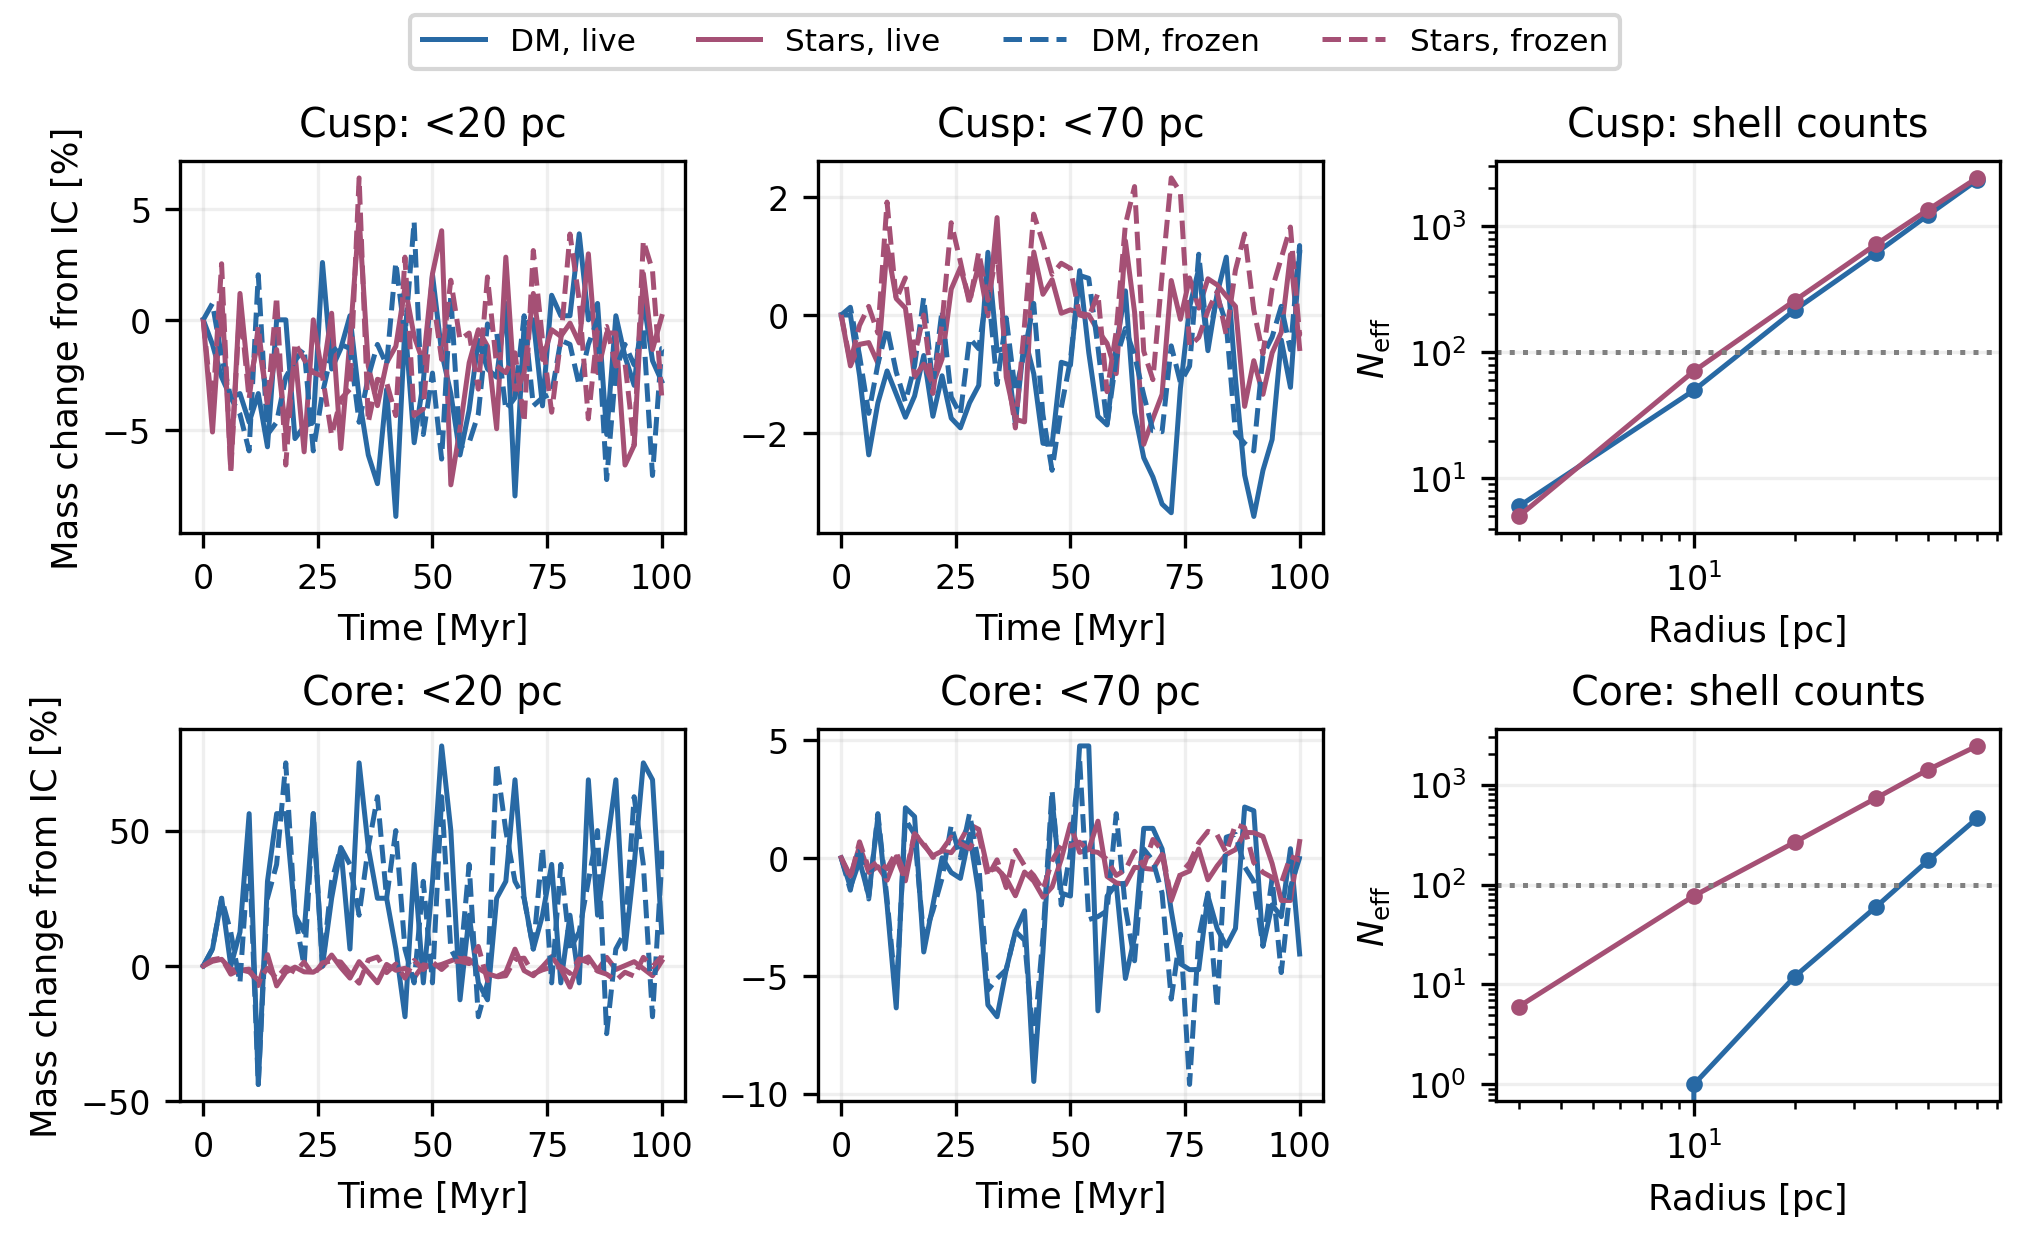
\includegraphics[width=\linewidth]{dynamical_batch_progenitor_isolation.png}
\caption{Progenitor isolation time series and effective shell counts. Blue
curves represent DM and purple curves stars; solid and dashed lines denote
live and frozen evolution. Left and middle columns show enclosed-mass changes
from each initial sample. The right column shows median live shell counts;
the dotted $N_{\rm eff}=100$ line is a visual reference, not a convergence
criterion. The cored halo's large central fluctuations occur in both engines
and coincide with very small DM counts.}
\label{fig:progenitor}
\end{figure}

\FloatBarrier
\section{Density changes at 20 pc across the batch}
\label{sec:density-summary}

Figure~\ref{fig:density-summary} collects all 24 completed evolutions in the
$18.1$--$22.1\pc$ shell, a local density diagnostic distinct from $\Mtwenty$.
Tidal runs are compared with matched isolation at the same time; isolation
runs are compared with their own initial samples.

The median tidal shell-density changes over the final $10\Myr$ are
$-2.50\%$ for both cusp engines, $-4.66\%$ for the live core and $-4.25\%$
for the frozen core. Doubled-$N$ remnants in isolation show median increases
of $0.35$--$0.77\%$ from their own initial densities. Their different particle
samples prevent attributing this sign change alone to particle number.

The progenitor cusp has median increases of $3.90\%$ and $6.59\%$ in its
live and frozen runs. The core's larger excursions remain unresolved with
only 15 initial effective shell particles. These results describe the
completed pilot configurations, including one tidal orbit.

\begin{figure}[htbp]
\centering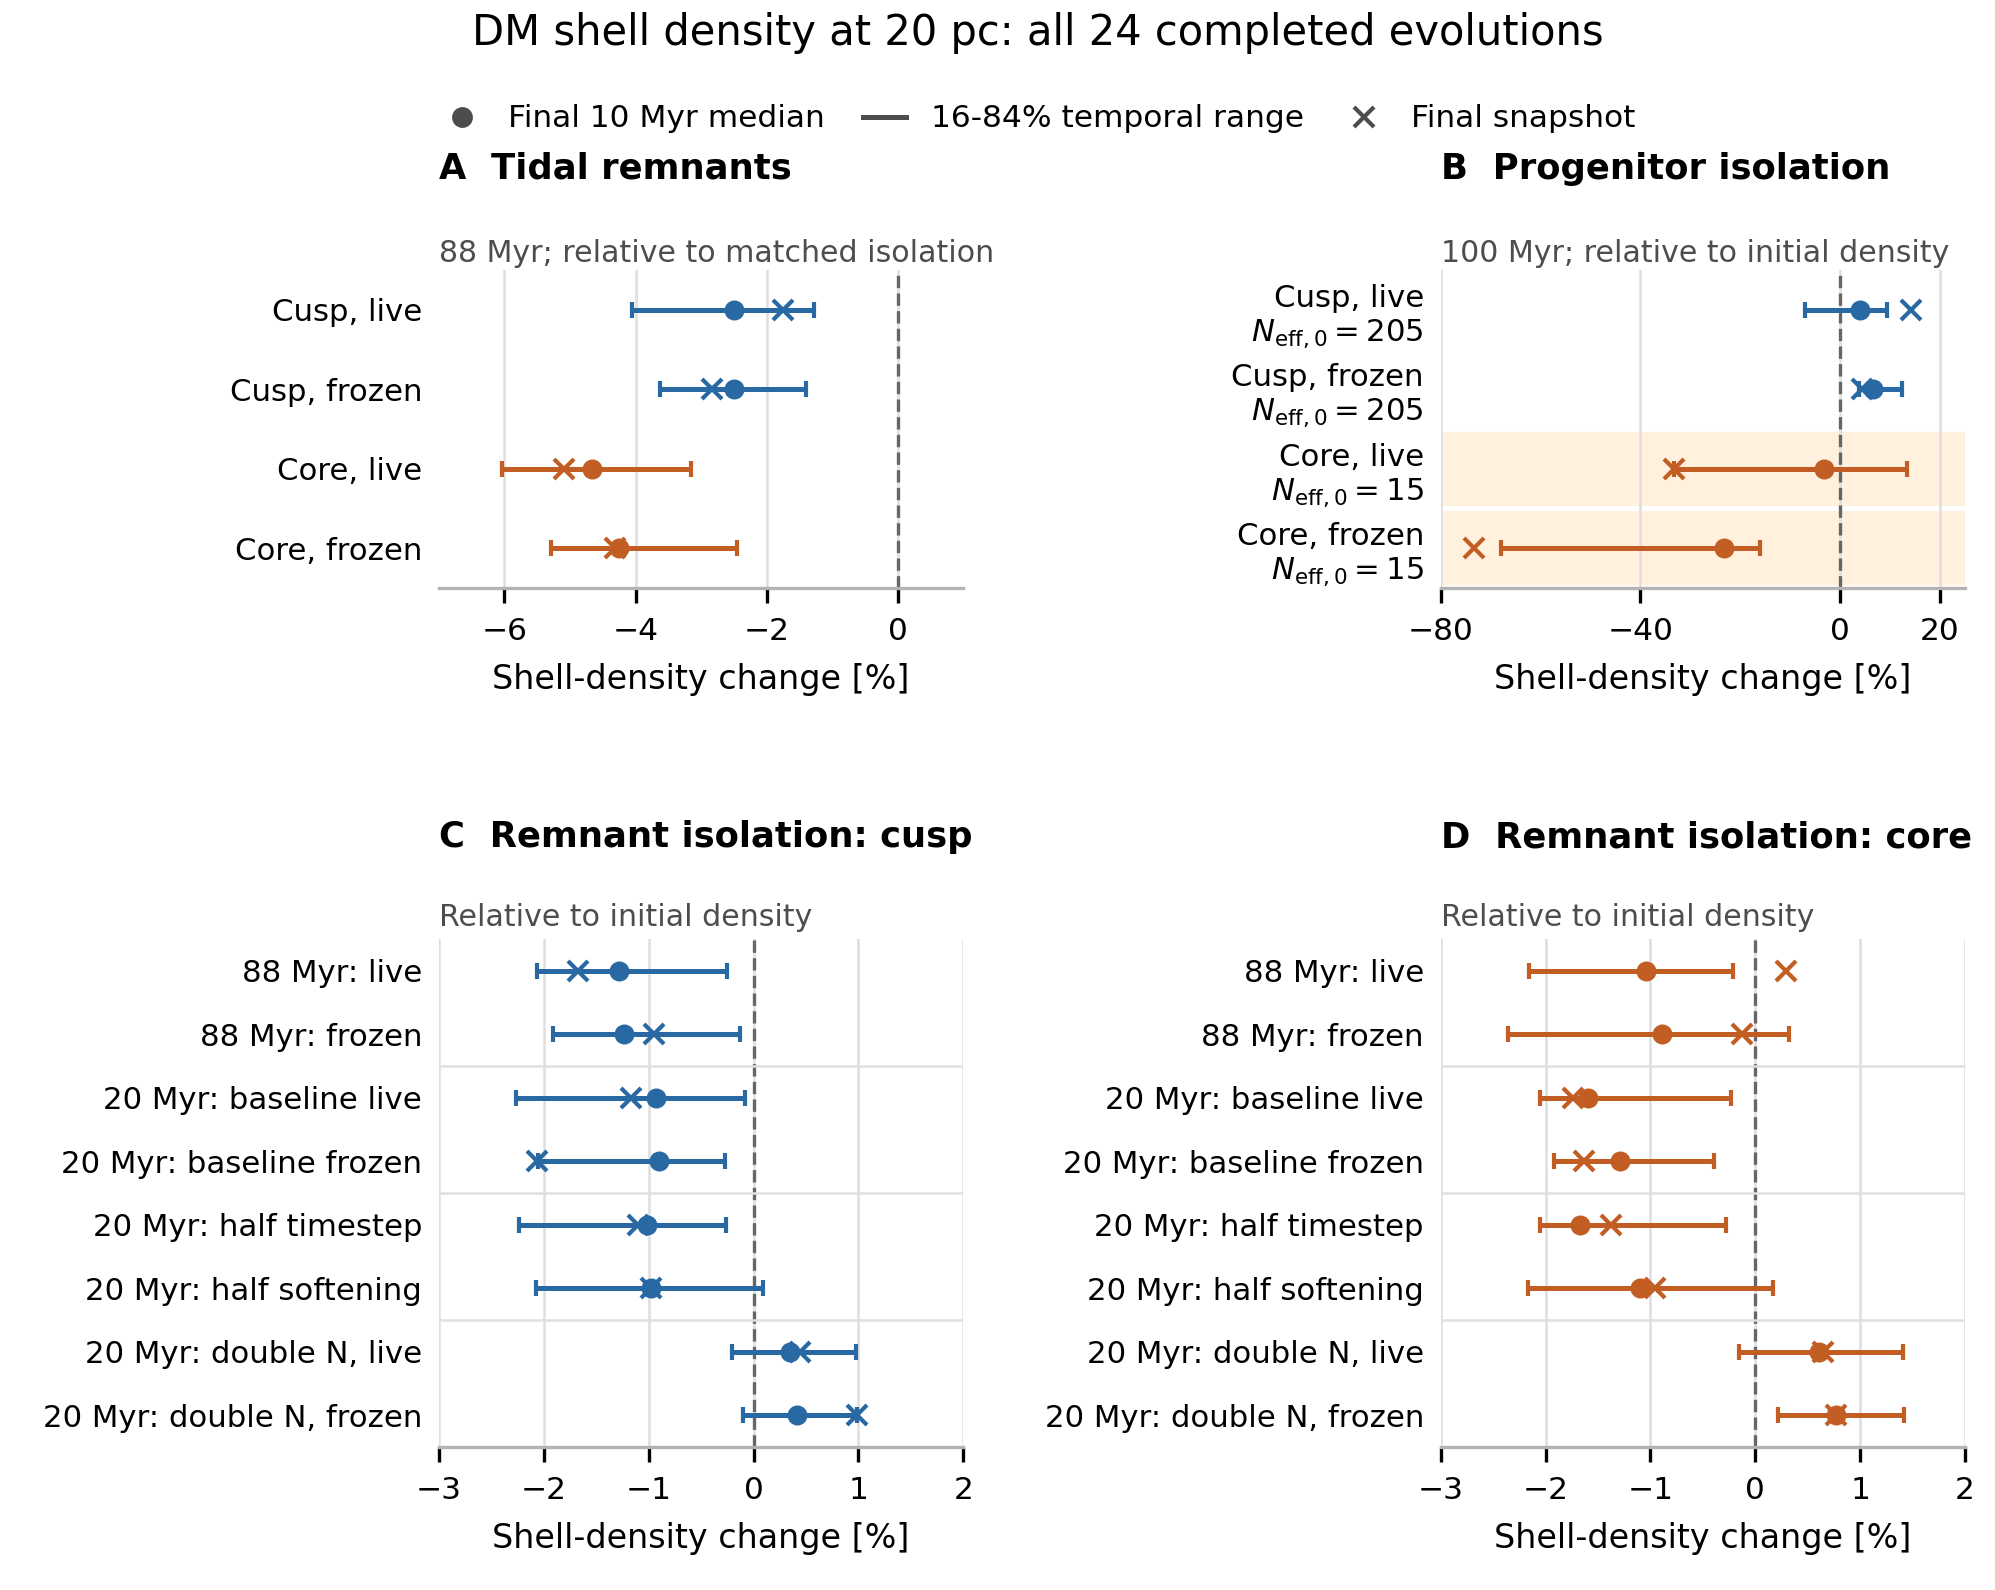
\includegraphics[width=\linewidth]{density_changes_20pc_paper.png}
\caption{DM shell-density changes at $20\pc$ across the full batch.
Blue denotes cusps and orange cores. Panel A shows the tidal effect relative
to matched isolation after one Galactic passage. Panels B--D show changes
from each run's own initial shell density; their durations are labelled.
Circles give medians over the final $10\Myr$, bars the temporal 16th--84th
percentiles, and crosses the final snapshot. The horizontal scales differ.
Shaded progenitor-core rows are unresolved at this radius; the labels give
initial effective shell counts. The lower panels include every completed
remnant isolation control, including the repaired half-softening cusp run.}
\label{fig:density-summary}
\end{figure}

\FloatBarrier
\section{What the batch supports and what comes next}

For the adopted compact models, one passage removes relatively little inner
DM while changing the outer density and anisotropy more strongly. The cored
distribution responds more strongly under the chosen inner-mass matching
convention. Disc-crossing timing offers a specific physical hypothesis for
part of the response. These results justify pursuing repeated-passage
survival, once numerical sensitivity has been checked under the full forcing.

The next remnant comparison should extend the timestep and particle-number
controls to the entire tidal interval, with corresponding isolation and
frozen controls and the repaired kernel. A second seed would measure
realisation variation that the temporal bands cannot. The $20$- and $70$-pc
responses should be assessed before expanding the physical grid. A later
comparison of host components could isolate the disc's contribution.

The progenitor programme can proceed independently towards an extended-body
disruption pilot on a specified orbit. Central-remnant measurements need
better sampling first, especially for the core. Simply doubling its present
particle number would leave only a few tens of DM particles inside $20\pc$;
the sampling design requires attention, followed by its own isolation check.
Diagnostics over $0.1$--$10\kpc$ at all output times should accompany the
next tidal runs.

All conclusions remain conditional on the imposed nucleus, orbit and initial
models. A self-consistent historical reconstruction would additionally need
the coupling of mass loss to orbital evolution and a responsive nucleus.
The current batch contains no progenitor tidal evolution and no repeated
remnant passages. No new simulation was launched to prepare this report.

\appendix
\section{Run provenance and reproduction}
\begingroup\small
\setlength{\parskip}{1pt}

The analysis comprises 24 completed evolutions from 14 preparations. It
excludes the original failed softening run, its unchanged repeat and its
instrumented failure. The successful replacement is
\path{remnant_cusp_eps_half/evolution_live_p1_fixed}.

The audit verified prepared inputs, all 24 diagnostic checksums, manifest
links, durations, monotonic times, mass invariance, nested apertures and matched
initial conditions and host/orbit files. Twelve independently read final
snapshots passed ID, mass and epoch checks and reproduced the saved aperture
masses. The expanded profile table has 264 rows; the analysis records 279
input hashes, including the snapshot files used in these measurements.

The principal project-relative locations are:
\begin{itemize}
 \setlength{\itemsep}{0pt}
 \item \path{results/dynamics/isolation_20260921T113007Z/}: baseline remnant
 and progenitor isolation runs.
 \item \path{results/dynamics/remnant_passage_20260921T114939Z/}: tidal runs,
 full-interval isolation references and numerical controls.
 \item \path{results/repairs/numerics_20260921T125417Z/}: force-kernel repair
 evidence, tests and successful replacement record.
 \item \path{results/dynamics/batch_analysis_20260921_v2/}: numerical summary,
 endpoint profiles, orbit context, analysis source copy and checksums.
\end{itemize}

The calculation is reproduced from the project root with
\path{bin/analyse_dynamical_batch.py}, using a fresh output directory:
{\small
\begin{verbatim}
export PYTHONPATH=src OMP_NUM_THREADS=1 OPENBLAS_NUM_THREADS=1
python bin/analyse_dynamical_batch.py \
  --output results/dynamics/batch_analysis_repeat
\end{verbatim}}
The pipeline and companion analysis are documented in
\path{docs/DYNAMICAL_EXPERIMENTS.md} and
\path{docs/DYNAMICAL_BATCH_ANALYSIS.md}.

Figure scripts are \path{bin/plot_dynamical_writeup.py},
\path{bin/plot_density_changes_20pc.py} and
\path{bin/plot_density_changes_20pc_paper.py}. JSON records in
\path{results/plot_data/} give their values and checksums; all required figures and provenance are
included in \path{output/source/dynamical_batch_latex.zip}.
The analytical comparisons are reproduced with
\path{bin/compare_dynamical_analytics.py}. Their three PNG figures and
\path{results/plot_data/dynamical_analytics.json} record the numerical values,
definitions and input hashes. The independent signed-DF inversion recovers
the input density to better than $2\times10^{-7}$ over the tested
$2.2$--$85\pc$ range. Doubling its energy grid and quadrature changes the
shell-retention fractions by less than $1.1\times10^{-7}$. Three independent
tests check the Kepler energy-cut limits and finite-shell integration.
Particle IDs, masses, matched times and audited snapshot hashes are checked
before the energy comparison; all existing simulation products are preserved.
Compile from \path{docs/} with \texttt{latexmk -pdf dynamical\_batch.tex}.
\endgroup

\begin{thebibliography}{9}
\bibitem{GHO1999} Gnedin, O.~Y., Hernquist, L., \& Ostriker, J.~P. 1999,
\emph{Tidal Shocking by Extended Mass Distributions}, ApJ, 514, 109--118;
\href{https://doi.org/10.1086/306910}{doi:10.1086/306910};
\href{https://arxiv.org/abs/astro-ph/9709161}{arXiv:astro-ph/9709161}.
\bibitem{GO1999} Gnedin, O.~Y., \& Ostriker, J.~P. 1999,
\emph{On the Self-consistent Response of Stellar Systems to Gravitational
Shocks}, ApJ, 513, 626--637;
\href{https://doi.org/10.1086/306864}{doi:10.1086/306864};
\href{https://arxiv.org/abs/astro-ph/9902326}{arXiv:astro-ph/9902326}.
\end{thebibliography}

\end{document}
